\section*{Overview of the appendices}
Appendices A--G document the profile source, H--J the learning source and K compute, software and licences. \Cref{tab:evidence} lists what each test showed and its main limit.

{\footnotesize\setlength{\tabcolsep}{4pt}\setlength{\LTcapwidth}{\linewidth}
\begin{longtable}{>{\raggedright\arraybackslash}p{3.0cm}>{\raggedright\arraybackslash}p{0.75cm}>{\raggedright\arraybackslash}p{1.9cm}>{\raggedright\arraybackslash}p{3.4cm}>{\raggedright\arraybackslash}p{3.5cm}}
\caption{What each test showed and its main limit. Status: P pre-specified test; R outcome registered before it was known;
H post hoc; E exploratory; D descriptive. Gains are pooled over the episodes of the set; pp: percentage points of
baseline-referenced gain.}\label{tab:evidence}\\
\toprule
Test & Status & Set & Result & Main limit\\
\midrule
\endfirsthead
\multicolumn{5}{l}{\emph{\tablename~\thetable, continued}}\\
\toprule
Test & Status & Set & Result & Main limit\\
\midrule
\endhead
\bottomrule
\endfoot
\multicolumn{5}{l}{\textbf{When to re-select profiles?} (\cref{sec:reselect})}\\
One-time gate against persistence (primary) & P & 2021, 98 episodes & $+0.504$\,pp $[+0.337, +0.704]$, pre-specified & the 20-episode extension gave $-0.004$\,pp, one of its episodes holding 22.5\% of its loss; families not resampled; a registered replication on 40 new episodes gave $+0.255$\,pp $[-0.037, +0.709]$, just short of its criterion; all 158 episodes $+0.366$\,pp $[+0.206, +0.535]$\\
Direction of the profile mismatch & H & 2021, 98 + 20 episodes & re-selection gained leaving the mild profile ($+11.1$\% on cold, $+3.5$\% on hot days) and lost entering it ($-6.5$\%, $-2.0$\%) & post hoc, on the episodes that tested the gate\\
\addlinespace
\multicolumn{5}{l}{\textbf{When to learn instead?} (\cref{sec:learn})}\\
Frozen profiles outside their families & P, D & development, held-out, leaderboard & gate $6.8$\,pp below G30; $-0.9$\% where G30 gained $4.1$\%; worse than $B$ & not run on the blind set\\
Learning on unseen architectures & P & blind, 12 architectures & $+2.82$\% over G30; 9 of 10 composite and both OOD improved & held-out: $+3.9$\% pooled but two of four composite improved (rule failed); one generator\\
The same layer on a later controller & P, R & ZT Best, blind & $+5.71$\% $[3.64, 7.55]$; all 12 improved & one further controller, with 41.6\% higher loss than K07-G30\\
Learning retargeted to energy & P & Penguin, blind & $+1.88$\% $[+1.12, +3.07]$; all 12 improved & a different mechanism (the start failed its gate)\\
The same layer on a trained neural controller & R & Residual PPO, blind & $+3.37$\% $[+1.57, +5.22]$; 8 of 10 composite improved; three of four registered predictions held & the pre-specified rule failed (two architectures lost 1.15 and 1.35\%)\\
The same layer on a graph network imitating the neural controller & R & blind & $+3.55$\% $[+1.82, +5.40]$; 8 of 10 composite improved; all four registered predictions held & imitates the neural controller (validation $R^2 \ge 0.97$); the pre-specified rule failed (52209 lost 1.17\%)\\
Each rule alone on the neural controller & R & Residual PPO, blind & pressure reset $+2.99$\% $[+1.60, +4.53]$, all 10 better; learned start $+0.49$\% $[-0.10, +1.03]$; all four registered predictions held & both losses of the layer came with the start; the new arms ran on another machine\\
Learning inside the full layer: learned against fixed time constant, both with the pressure reset & R & blind, K07-G30 & $+0.94$\% $[+0.10, +1.82]$; 7 of 10 composite better & exact Wilcoxon $p = 0.084$: stronger for the pooled gain than per architecture\\
Knowing the time constant from day~1 (oracle) & R & blind, K07-G30 & $+0.02$\% $[-0.003, +0.057]$ over the layer, mostly in days 1--14 & the value of knowing $\tau$ early, not a general upper bound; not deployable\\
\addlinespace
\multicolumn{5}{l}{\textbf{When does the layer help?} (\cref{sec:when,sec:lb})}\\
Account of the gain (headroom) & H, R & blind; ZT registered & $\rho = 0.80$, not an artefact of the shared denominator; five of seven predictions registered for two controllers held & post hoc; weak for Penguin across architectures\\
Time to value; early indication & H, E & blind, 30 composite episodes & learned start ahead of the fixed one from day~6; first-week comfort share ranked the later gain ($\rho = 0.72$) & post hoc and exploratory; not a selector\\
A third rule: the unoccupied setup added to the layer & R & blind, K07-G30 & $+0.38$\% $[-0.45, +1.49]$; energy and carbon down, comfort up & not tuned for the combination\\
Unoccupied setup (from a diagnosis of the official scenes) & P, R & development, official scenes, blind & passed its gate; leaderboard 4.3\% below G30; on the blind set $-0.62$\% alone, $+1.27$\% with the learned start & the pre-specified rule failed (one architecture lost 3.3\%); the official scenes informed the design\\
Leaderboard & D, R & hidden scenes & learning unchanged on K07 and 1.0\% worse on the neural controller (registered: no change); Penguin with precooling nearly unchanged; the unoccupied setup 4.3\% better; the gate worse than $B$ & official scenes' comfort share 0.2--4.6\%; one set of scenes\\
\end{longtable}}

%======================================================================
\section{Cohorts, weather references and study lineage}\label{app:cohorts}
%======================================================================
\paragraph{Common design.}
An episode pairs one generated building variant with one historical weather window and a declared scoring horizon; matched
policies share these inputs. Repeated windows, stations and parent-building families create dependence, so cohorts are
analysed separately and their sample sizes are not additive; the 2021 main, extension and replication episodes are distinct
but share stations and families, and they are pooled only in a registered secondary analysis (\cref{app:inference}). Initial weather strata use the file-derived mean temperature
over the first 19 hours and the thresholds of \cref{sec:profilesource}; the class observed by the running policy, from its
first 228 five-minute temperatures, can differ from this design stratum. An early three-class reference (1,836 eligible
Sunday starts at 36 stations) grouped all temperatures below 11\,$^\circ$C as cold; the later four-class reference (1,872
starts) separates extreme cold (\cref{tab:ref}). Eligibility required at least 72 hourly observations and did not guarantee
that a window could support a full 30-day rollout. The 2023 analysis weights each stratum by its reference mass, distributed
equally among the sampled episodes of that stratum; the 2022 and 2021 analyses use equal cell weights in the pooled losses.

\begin{table}[!htbp]
\centering
\caption{Initial-weather reference counts and the 2023 evaluation sample. Reference counts are eligible source windows,
not evaluated episodes.}
\label{tab:ref}
\small
\begin{tabular}{lrrr}
\toprule
Initial class & Three-class reference & Four-class reference & 2023 episodes\\
\midrule
Extreme cold (E) & included in C & 17  & 0\\
Cold (C)         & 569           & 574 & 23\\
Mild (M)         & 801           & 814 & 24\\
Hot (H)          & 466           & 467 & 23\\
\midrule
Total            & 1,836         & 1,872 & 70\\
\bottomrule
\end{tabular}
\end{table}

\paragraph{What differs between studies.}
\Cref{tab:lineage} lists each study with what sets it apart, and \cref{fig:timeline} gives their order. The first-workday and
five-day studies established the baseline and the profiles and exposed weather-dependent failures; they are not independent
30-day validations. The 2021 test used hourly NOAA ISD weather for 2021~\cite{smith2011isd}, a year not used before. Its
frozen window screen required a 720-hour window, starts at least 35 days apart at a station and at most three windows per
station; its 42 stations were 30 from the earlier pool and 12 from the additional-station 2022 cohort. The gate, six arms,
episode order, primary contrast and analysis were frozen in an internal, time-stamped protocol before any 2021 rewards were
inspected; a later amendment changed only retry handling after initialisation failures.

\begin{figure}[!htbp]
\centering
\resizebox{\linewidth}{!}{\begin{tikzpicture}[
  font=\small,
  st/.style={draw, rounded corners=2pt, align=center, text width=23mm, minimum height=20mm, inner sep=3pt},
  exp/.style={st, fill=black!4, draw=black!50},
  conf/.style={st, fill=green!8, draw=green!45!black, very thick},
  frz/.style={st, fill=white, draw=green!45!black, dashed, text width=19mm},
  arr/.style={-{Latex[length=2mm]}, thick, black!60}
]
\node[exp]  (d)  {\textbf{Development}\\[1pt]\scriptsize first-workday \& 5-day studies; baseline $B$, profile library, G30};
\node[exp,  right=4mm of d]  (a) {\textbf{2023 weather}\\[1pt]\scriptsize $n=70$ (23/24/23)\\ fixed vs.\ schedules; sparse \& persistence arms added};
\node[exp,  right=4mm of a]  (b) {\textbf{2022 weather}\\[1pt]\scriptsize $n=58$ and $n=30$\\ frozen schedules; mild-start pattern observed};
\node[frz,  right=4mm of b]  (f) {\textbf{Internal freeze}\\[1pt]\scriptsize gate MG, 6 arms, sample order, primary contrast, analysis};
\node[conf, right=4mm of f]  (t) {\textbf{2021 weather}\\[1pt]\scriptsize $n=98$ main\\ (+20 optional)\\ primary test};
\foreach \u/\v in {d/a, a/b, b/f, f/t} \draw[arr] (\u) -- (\v);
\draw[decorate, decoration={brace, mirror, amplitude=5pt}, black!60]
  ([yshift=-2mm]d.south west) -- node[below=6pt, font=\scriptsize]{exploratory: outcomes inspected, policies revised} ([yshift=-2mm]b.south east);
\draw[decorate, decoration={brace, mirror, amplitude=5pt}, green!45!black]
  ([yshift=-2mm]f.south west) -- node[below=6pt, font=\scriptsize, text=green!35!black]{pre-specified, outcomes unseen} ([yshift=-2mm]t.south east);
\end{tikzpicture}
}
\caption{Study chronology. Exploratory stages (grey) informed the profile library and, after the 2022 results, the
one-time gate. The gate, six policy arms, episode order, primary contrast and analysis were then frozen before the
2021 evaluation (green). A replication registered before its runs then added 40 new 2021 episodes (\cref{app:inference}).}
\label{fig:timeline}
\end{figure}

\begin{table}[!htbp]
\centering
\caption{Study lineage: what sets each study apart. Added arms, nested horizons and reused windows do not create new
independent samples. C/M/H: cold/mild/hot by design.}
\label{tab:lineage}
\footnotesize
\begin{tabular}{>{\raggedright\arraybackslash}p{2.7cm}>{\raggedright\arraybackslash}p{1.25cm}>{\raggedright\arraybackslash}p{8.7cm}}
\toprule
Study & Episodes & What sets it apart\\
\midrule
Early first-workday screen & 240 & 120 windows at 36 stations, each paired with two of 56 building variants; non-random selection: spring under-represented, temperatures near 11\,$^\circ$C excluded\\
Later first-workday selection & 202 & 204 planned, two all-arm failures; weather-based selection reconstructed offline from recorded static-policy outcomes, not executed as a multi-day controller\\
Direct five-day / nested 30-day & 80 / 36 & the 36 with enough weather for a nested 30-day evaluation belong to the 80\\
2023 30-day comparison & 70 & 72 planned in two tranches of 36; one cold and one hot case of the second failed to initialise in all arms; 70 distinct windows at 30 stations; five arms at first ($B$, an alternative fixed profile, select-once, daily, predefined-day)\\
Additional fixed / sparse arms & 70 (reused) & four fixed profiles and two sparse schedules on the same 70 episodes, eleven arms in all; in 11 hot-start episodes the original and added arms ran on different machines without demonstrated numerical parity, the other 59 on one machine each\\
Extreme-cold diagnostics & 34 / 13 & five-day cases; the 13 longer cases reuse earlier windows\\
2022 cohorts & 58 / 30 & previously unevaluated 2022 weather; new variants of the same six families; six arms ($B$, two fixed alternatives including G30, select-once, daily, persistence); 27 previously used / 13 additional stations; the first ran 60 episodes, and two pilots whose outcomes had been examined were excluded\\
2022 post-outcome cohort & 30 & specified afterwards; exploratory; 20 stations\\
2021 main / optional & 98 / 20 & pre-specified test at 42 / 17 stations; 100 main planned, half on variants seen under 2022 weather and half on new ones; two new variants failed in all six arms and were excluded without replacement (50 reused, 48 new); C/M/H 30/42/26 and 6/9/5\\
2021 registered replication & 40 & registered before its runs (\cref{tab:registry}); arms $B$, TRIG2 and MG; 28 stations; C/M/H 12/18/10; no episode overlaps an earlier one (\cref{app:inference})\\
\bottomrule
\end{tabular}
\end{table}

%======================================================================
\section{Reward components and stratum contributions in earlier studies}\label{app:components}
%======================================================================
The later 30-day cohorts archived total loss but not complete component series. Component evidence is available only for
two earlier first-workday studies, which used a shorter horizon and selected offline, by the initial weather label, among
separately recorded fixed-policy trajectories. Because alternative profiles can change settings that act before the first
decision, this is not equivalent to a causal controller that starts under $B$ and then switches; the 30-day cohorts were
executed in closed loop. For a cohort with strata $k$, reference masses $F_k$ and within-stratum mean components
$\bar q_{a,k}, \bar c_{a,k}, \bar e_{a,k}$ for policy $a$,
\begin{equation}
  L_{a} = \sum_k F_k\,(0.6\,\bar q_{a,k} + 0.2\,\bar c_{a,k} + 0.2\,\bar e_{a,k}),
  \qquad G_{a/B} = 100\,(1 - L_a/L_B).
\end{equation}
A common normalisation of the reference masses cancels in this ratio.

\paragraph{Early two-action offline selection.}
On 240 first-workday episodes, a rule selecting $B$ below 11\,$^\circ$C and an alternative configuration otherwise
reduced aggregate loss by 1.21\%, with energy and carbon terms down 1.69\% and 1.94\%, but increased reference-weighted
comfort regret by 15.99\%: unchanged after cold starts, up by 116\% after mild and 479\% after hot ones, from small bases. Regret increased in 72 episodes, decreased in 16 and was unchanged in 152;
the 16 episodes with more than 1\% higher loss (3 mild, 13 hot) all had higher regret.

\paragraph{Four-regime offline selection.}
On 202 first-workday episodes (E/C/M/H $=$ 67/47/48/40), selecting the profile by four-class weather reduced loss by
5.46\%, energy cost by 4.77\%, carbon by 5.86\% and comfort regret by 8.14\%. Mean regret fell by 10, 15 and 25\% in the extreme-cold, cold and hot strata,
but in the mild stratum it increased by 121\% from a small base despite lower total loss. Nine episodes
exceeded the 1\% loss-deterioration threshold (seven extreme-cold, two mild), all with increased regret.

\paragraph{Contribution by stratum (2023 cohort).}
Without component series, the 2023 gain can still be decomposed by initial stratum. With $S_{B,k} = 100F_kL_{B,k}/L_B$
the baseline-loss share and $D_k = 100F_k(L_{B,k}-L_{\mathrm{daily},k})/L_B$ the contribution to daily re-selection's
gain, cold episodes contribute most (2.05 of the 4.36\pp; mild 1.60, hot 0.71) because they carry the largest share of
baseline loss (47\%, against 26\% each for mild and hot, at reference masses of 31, 44 and 25\%). This is a contribution to the gain over $B$; the advantage of daily
re-selection over select-once, a different comparison, is concentrated in mild episodes (\cref{app:extended}).

%======================================================================
\section{Extended comparisons and development evidence}\label{app:extended}
%======================================================================
\paragraph{2023 cohort: fixed and sparse policies.}
\Cref{tab:2023} reports all policies on the 70 episodes and \cref{tab:2023class} the gains by initial class.
Persistence retained most of daily re-selection's gain (4.24\% against 4.36\%) with about half the changes (1.99 against
3.93 per episode); predefined-day and weekly schedules
also improved on $B$ with fewer changes. GL, the strongest of the originally tested fixed profiles, and G30 both came
close to the adaptive schedules. In mild-start episodes, daily re-selection exceeded select-once by 4.48\pp, compared
with 0.15\pp{} in cold and 0.28\pp{} in hot starts. Two development profiles derived for cold weather, INC and WS1,
improved loss in cold-start episodes but incurred about 52\% higher loss than $B$ in hot-start episodes (\cref{tab:transfer};
HOTINC was derived for hot weather). These selected failures of a mismatched regime do not estimate an unconditional failure
rate or test transfer to new buildings, but they show why profile choice must be conditioned on the regime. In 11 hot-start
episodes the original and added arms ran on different machines without demonstrated numerical parity (\cref{tab:lineage}).

\begin{table}[!htbp]
\centering
\setlength{\tabcolsep}{4pt}
\begin{minipage}{0.46\linewidth}\centering
\caption{2023 cohort ($n=70$, reference-weighted). Changes: post-initial profile changes per episode, from the logs of
2,100 daily windows per policy (in total PD5 275, LIST 117, WEEK 71, TRIG2 139).}
\label{tab:2023}
\footnotesize
\begin{tabular}{lrr}
\toprule
Policy & Gain (\%) & Changes\\
\midrule
$B$                        & 0.00     & 0\\
A1 (alternative fixed)     & $-3.48$  & 0\\
GL (earlier tuned fixed)   & $+3.53$  & 0\\
G30 (30-day tuned fixed)   & $+3.60$  & 0\\
PS5 (select once)          & $+3.03$  & 0\\
PD5 (daily)                & $+4.36$  & 3.93\\
LIST (predefined days)     & $+4.01$  & 1.67\\
WEEK (weekly)              & $+3.91$  & 1.01\\
TRIG2 (persistence)        & $+4.24$  & 1.99\\
\bottomrule
\end{tabular}
\end{minipage}\hfill
\begin{minipage}{0.5\linewidth}\centering
\caption{2023 cohort: gain (\%) by initial class. The overall gains of \cref{tab:2023} weight the classes by
their shares of the baseline loss (\cref{app:components}), not equally.}
\label{tab:2023class}
\footnotesize
\begin{tabular}{lrrrrr}
\toprule
Class ($n$) & PS5 & PD5 & GL & WEEK & TRIG2\\
\midrule
Cold (23) & 4.17 & 4.32 & 4.08 & 3.97 & 4.26\\
Mild (24) & 1.59 & 6.07 & 2.79 & 5.06 & 5.76\\
Hot (23)  & 2.42 & 2.70 & 3.28 & 2.63 & 2.66\\
\bottomrule
\end{tabular}
\vspace{6pt}
\caption{Fixed profiles across initial weather classes: gain (\%) versus $B$ (selected cross-regime failures).}
\label{tab:transfer}
\begin{tabular}{lrrrr}
\toprule
Profile & Cold & Mild & Hot & All\\
\midrule
INC (cold)    & 4.15 & 2.53 & $-51.84$ & $-10.93$\\
WS1 (cold)    & 4.61 & 2.05 & $-51.79$ & $-10.82$\\
HOTINC (hot)  & 0.40 & $-0.97$ & 2.42 & 0.56\\
\bottomrule
\end{tabular}
\end{minipage}
\end{table}

\paragraph{2022 cohorts.}
\Cref{tab:2022} gives the two 2022 cohorts of frozen schedules. In mild starts, daily re-selection gained 4.92\% against
1.54\% for select-once at previously used stations and 4.57\% against $-0.92$\% at additional stations; this mild-start
pattern was identified after these outcomes were examined.

\begin{table}[!htbp]
\centering
\caption{2022 cohorts of frozen schedules (equal cell weights; 95\% station-cluster intervals).}
\label{tab:2022}
\small
\begin{tabular}{lcc}
\toprule
Cohort & Daily vs.\ $B$ (\%) & Daily $-$ once (pp)\\
\midrule
Previously used stations ($n = 58$) & $+4.29$ $[+3.32, +5.42]$ & $+0.56$ $[+0.06, +1.18]$\\
Additional stations ($n = 30$)      & $+3.25$ $[+1.88, +4.75]$ & $+1.49$ $[+0.17, +3.02]$\\
\bottomrule
\end{tabular}
\end{table}

\paragraph{Context--parameter associations.}
During development, high and low values of nine controller parameters around an early configuration were compared on
24 first-workday episodes. Six directional hypotheses linking parameter preferences to weather or building properties
were then specified and tested on 24 new episodes with family-centred Spearman correlations, 20,000 within-family
permutations and Benjamini--Hochberg control~\cite{benjamini1995fdr} at $q=0.10$. Three of the four hypotheses on the
19-hour temperature met this exploratory criterion; the fourth and both wall-density hypotheses did not (\cref{tab:assoc}).
These associations informed development; they do not validate the profiles.

\begin{table}[!htbp]
\centering
\setlength{\tabcolsep}{4pt}
\caption{Development-stage association tests ($\rho$: initial and replication samples; $p$ and $q_{\mathrm{BH}}$ from the
replication; pass: $q_{\mathrm{BH}} \le 0.10$). $T_{19}$: mean outdoor temperature over the first 19\,h; wall density: density
of the interior-wall material in the building's configuration.}
\label{tab:assoc}
\footnotesize
\begin{tabular}{lrrrrc}
\toprule
Context $\times$ parameter & $\rho_1$ & $\rho_2$ & $p$ & $q_{\mathrm{BH}}$ & Pass\\
\midrule
$T_{19}$ $\times$ PRESTART\_H        & $-.40$ & $-.42$ & .0357 & .0714 & yes\\
$T_{19}$ $\times$ EVENING\_STOP\_H   & $-.32$ & $-.46$ & .0249 & .0714 & yes\\
$T_{19}$ $\times$ MILD\_SHIFT\_K     & $-.30$ & $-.74$ & .0001 & .0006 & yes\\
$T_{19}$ $\times$ HEAT\_U\_SCALE     & $-.28$ & $-.15$ & .2620 & .3930 & no\\
Wall density $\times$ KI             & $+.40$ & $-.16$ & .7404 & .7404 & no\\
Wall density $\times$ EVENING\_STOP\_H & $-.05$ & $-.06$ & .5939 & .7127 & no\\
\bottomrule
\end{tabular}
\end{table}

\paragraph{Exploratory threshold search.}
An offline analysis reusing the 2023 fixed-arm outcomes cross-validated one to four temperature partitions and chose a
fixed profile per partition. A three-segment fit (cuts near 1.5 and 21.6\,$^\circ$C) gave a cross-validated gain of
5.17\% versus $B$, compared with 2.28\% for the hand-set partition under the same procedure. Because the number of
segments was chosen after inspecting the scores and the episodes were reused, the 5.17\% is exploratory and potentially
selection-biased; it does not establish better thresholds for a prospectively evaluated, closed-loop selector.

%======================================================================
\section{Execution and quality assurance}\label{app:execution}
%======================================================================
\paragraph{Decision rule.}
The selector uses $\bar T_d$ at step $t_d$ as defined in \cref{sec:profilesource}; the first decision falls on Monday 01:00.
If the window lacks any of its 228 observations, the current profile is retained; at the first decision this leaves $B$
active. The controller also retains its own extreme-cold logic based on an exponential moving average of outdoor air
temperature, which can respond at a different time from the external selector.

\paragraph{Profile application.}
At an adoption, all parameters that any profile may override are set to the target profile's values or to the
baseline/constructor defaults. A persistent internal attribute storing the pre-start time is synchronised with the
pre-start parameter; an early pilot showed that without this step the controller could revert to an obsolete setting
(25 of 126 checks failed before the fix; 189 of 189 passed after it, with bitwise parity over 480 steps on nine pilot
cases). This restoration is deterministic but is not a proof of bumpless transfer.

\paragraph{2021 gate execution and QA.}
In the 98 main episodes, 43 entered the mild (daily) branch and 55 the select-once branch; three observed classes
differed from the design labels. All 98 gate losses equal exactly the loss of the corresponding PD5 or PS5 arm (maximum
relative difference zero). Before inspecting 2021 rewards, six previously evaluated 2022 episodes (two per regime) were re-run: the
gate reproduced its branch in rewards, actions, decisions and logs on two local hosts. The hosted runtime was not
bitwise identical; a pre-declared tolerance screen admitted it (on the six re-run episodes the gate had to match the corresponding
PD5 or PS5 result within 0.5\%, with a spread across machines of at most 2\%; mean hosted-minus-local difference in the
primary contrast $-0.024$\pp, maximum absolute $0.270$\pp). By environment, the primary contrast was $+0.482$\pp{} on local host A (54 episodes), $+0.633$\pp{} on the hosted runtime
(24) and $+0.379$\pp{} on local host B (20); because different episodes ran on each, these are not paired hardware comparisons.

\paragraph{Registration record.} Every registered test was frozen in a protocol before its runs (\cref{tab:registry}). The
repository's integrity folder holds the append-only ledger in which each protocol's SHA-256 was recorded before the outcome it
concerns, a map from each published copy (working notes and local paths removed) to the hash of its original, and
OpenTimestamps proofs for the registrations from 11 November evening onwards (OTS). The ledger records internal freezes;
only the registrations marked OTS also carry independent timestamp evidence.
\begin{table}[!htbp]
\centering
\caption{Registration record: each registered test, its protocol in the repository, when it was frozen (EET, as written in the
protocol; day only where the protocol gives none) and the first 12 hexadecimal digits of the SHA-256 of the original protocol.
OTS: also stamped with OpenTimestamps.}
\label{tab:registry}
\scriptsize
\setlength{\tabcolsep}{3pt}
\begin{tabular}{>{\raggedright\arraybackslash}p{3.5cm}>{\raggedright\arraybackslash}p{4.7cm}lll}
\toprule
Test & Protocol (\path{experiments/}) & Frozen & SHA-256 & OTS\\
\midrule
One-time gate, 2021 & \path{01_profile_study_2021/PROTOCOL.md} & 8 Nov 02:59 & \texttt{9a566eb3859f} & \\
Learned start, development gate & \path{02_development_gates/k07_learned_start/PROTOCOL.md} & 10 Nov 12:49 & \texttt{f43b77bfa249} & \\
Pressure reset, development gate & \path{02_development_gates/k07_pressure_reset/PROTOCOL.md} & 10 Nov & \texttt{5bfc700c7ba0} & \\
Layer on unseen architectures & \path{04_blind_set_k07/PROTOCOL.md} & 10 Nov 15:46 & \texttt{51e00be89a35} & \\
$B$ and fixed start on the same scenes & \path{03_out_of_family_and_held_out/layer_held_out/PROTOCOL.md} & 11 Nov 01:30 & \texttt{fb1d5273fc5e} & \\
Penguin with learned precooling & \path{06_penguin_precooling/PROTOCOL.md} & 11 Nov 00:47 & \texttt{65184e4aa16f} & \\
Unoccupied setup & \path{08_unoccupied_setup/PROTOCOL.md} & 11 Nov 10:26 & \texttt{9e20135bf6a3} & \\
ZT Best and its headroom predictions & \path{05_maintenance_zt_best/PROTOCOL.md} & 11 Nov 11:05 & \texttt{c96cb145ddac} & \\
Residual PPO and its predictions & \path{07_neural_controller/PROTOCOL.md} & 11 Nov 21:02 & \texttt{2c6a414e36a6} & OTS\\
Graph network & \path{09_graph_network_controller/PREREG_GNNSUP_v1.md} & 12 Nov & \texttt{317beada4d12} & OTS\\
Oracle start, third rule, rule ablation & \path{10_extension_ablation_oracle_rules/PROTOCOL.md} & 12 Nov & \texttt{af3a09532096} & OTS\\
Replication of the 2021 gate test & \path{12_replication_2021/PROTOCOL.md} & 12 Nov 12:57 & \texttt{250d354a3f67} & OTS\\
Fixed time constant inside the layer & \path{13_learning_inside_the_layer/PROTOCOL.md} & 12 Nov 13:45 & \texttt{d27dabbad43b} & OTS\\
\bottomrule
\end{tabular}
\end{table}

%======================================================================
\section{Inference details and sensitivity}\label{app:inference}
%======================================================================
\paragraph{2021 primary analysis.}
The estimand is the pooled-loss gain of \cref{eq:delta} with $S$ the 98 main episodes and equal cell weights. The 42 station identities are
resampled with replacement 3,000 times (fixed seed), retaining all episodes and arms of each sampled station; the 2.5th
and 97.5th percentiles form the interval. The analysis uses the class observed at the first decision, which differs from the weather-file label in three episodes. \Cref{tab:sens} collects the sensitivity analyses.

\paragraph{Primary contrast and regime classes: further detail.}
Expressed as a direct loss reduction between the two schedules, the primary contrast corresponds to 0.525\%; the gate had
lower loss than persistence in 58 episodes, higher loss in 15 and identical loss in 25. Decomposed by the branch actually
taken, the 55 non-mild episodes (following select-once) contributed $+0.339$\pp{} and the 43 mild episodes (following
daily) $+0.165$\pp; within each branch the gate exceeded persistence by $+0.465$ and $+0.609$\pp{} respectively, and the
non-mild branch contributes more in aggregate because it carries a larger share of baseline loss. On 2021 weather, with
the weather-file label as the class, the gains of select-once, daily re-selection and the gate versus $B$ were 4.96, 4.63 and 5.08\% after cold starts, 1.81,
4.40 and 4.41\% after mild starts, and 2.71, 2.44 and 2.89\% after hot starts.

\paragraph{Robustness.}
The primary contrast survived re-weighting by historical regime frequencies, restriction to subsets of building
variants, another source of class labels and leaving out one station or family (\cref{tab:sens}). These checks show how
much the estimate depends on single stations or families; they do not model the dependence between variants of a family.

\paragraph{The 20-episode extension (post hoc reading).}
The pre-specified 20-episode extension gave $-0.004$\pp; \cref{tab:sens} also gives it pooled with the main sample, as the
protocol reports it. Read after its outcome, it had the main sample's mix of starts (9 of its 20 episodes started mild, as
did 43 of the 98) but one dominant episode: a cold January start in Kansas City held 22.5\% of its baseline loss, and there
the gate trailed persistence by 1.26\pp. Per episode the gate gained in 10 of the 20, lost in 7 and tied in 3; its mean
episode-wise gain, a different estimand that averages each episode's own percentage gain and is not a re-weighting of the
primary one, was $+0.314$\pp{} $[-0.098, +0.887]$, against $+0.627$\pp{} in the main sample. The primary estimand is a
pooled-loss gain, a ratio of losses summed over episodes: every episode counts once, but an episode with a larger baseline
loss weighs more in the percentage. Its loss-weighted effective number of episodes, $n_{\mathrm{eff}} = (\sum_e L^{B}_e)^2/\sum_e
(L^{B}_e)^2$, is 54.5 of the 98 main episodes but only 9.8 of the 20 extension episodes; it measures how concentrated the
baseline loss is, not a sample size adjusted for shared stations or families. The extension's interval, computed
post hoc in the same way as the primary one, contains the main estimate, so the extension neither confirms nor contradicts
it: twenty episodes with one dominant episode are compatible with a modest effect and with none. The effect is modest and
not uniform.

\paragraph{Registered replication.}
A replication registered before its runs (\cref{tab:registry}), on 40 new 2021 episodes at 28 stations, none overlapping an
earlier episode, gave $+0.255$\pp{} (the gate 4.06\% and persistence 3.81\% over $B$; interval in \cref{tab:sens}). Its
estimate is positive and 95\% of its bootstrap resamples lie above zero (post hoc), but its interval just includes zero, so
it falls just short of the registered criterion for replication, a lower bound above zero, and far from the criterion for
failure, an upper bound below $+0.25$\pp; by its rule it is inconclusive. Its mean episode-wise gain was $+0.517$\pp{}
$[+0.076, +1.125]$ (the gate better in 16 episodes, worse in 6, tied in 18), and no episode held more than 12.2\% of its
baseline loss (without that one, $+0.291$\pp). Pooled over all 158 episodes of the main sample, the extension and the
replication (42 stations), a secondary analysis registered with it, the gate gained $+0.366$\pp{} (\cref{tab:sens}).

\begin{figure}[!htbp]
\centering
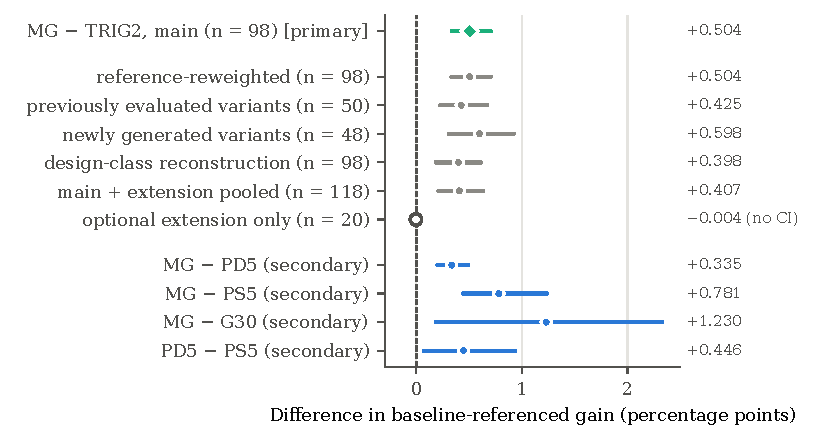
\includegraphics[width=\linewidth]{figures/fig_contrasts_col.pdf}
\caption{Paired differences in baseline-referenced gain on 2021 weather with 95\% station-cluster intervals. Top:
pre-specified primary contrast. Middle: sensitivity analyses of the same contrast (the 20-episode extension is shown
without its post hoc interval, given in \cref{tab:sens}). Bottom: secondary contrasts (Holm-adjusted $p$-values in \cref{tab:secondary}).}
\label{fig:contrasts}
\end{figure}

\begin{table}[!htbp]
\centering
\caption{2021 primary contrast (MG $-$ TRIG2, pp): main estimate and sensitivity analyses.}
\label{tab:sens}
\small
\begin{tabular}{lrrc}
\toprule
Analysis & $n$ & $\Delta$ (pp) & 95\% interval\\
\midrule
Primary: pooled-loss gain                  & 98  & $+0.504$ & $[+0.337, +0.704]$\\
Mean episode-wise gain (post hoc)          & 98  & $+0.627$ & $[+0.414, +0.841]$\\
Reference-mass re-weighting                & 98  & $+0.504$ & $[+0.333, +0.706]$\\
Previously evaluated building variants     & 50  & $+0.425$ & $[+0.227, +0.671]$\\
Newly generated building variants          & 48  & $+0.598$ & $[+0.306, +0.921]$\\
Gate reconstructed from design labels      & 98  & $+0.398$ & $[+0.183, +0.613]$\\
Optional extension only (interval post hoc) & 20 & $-0.004$ & $[-0.451, +0.705]$\\
Extension without its largest episode (post hoc) & 19 & $+0.359$ & ---\\
Main and extension pooled                  & 118 & $+0.407$ & $[+0.210, +0.633]$\\
Main and extension, mean episode-wise gain (post hoc) & 118 & $+0.574$ & $[+0.379, +0.779]$\\
Registered replication, new episodes        & 40  & $+0.255$ & $[-0.037, +0.709]$\\
All 158 episodes pooled (registered secondary) & 158 & $+0.366$ & $[+0.206, +0.535]$\\
Leave-one-station-out (range)              & --- & \multicolumn{2}{l}{$+0.462$ to $+0.544$}\\
Leave-one-family-out (range)               & --- & \multicolumn{2}{l}{$+0.413$ to $+0.591$}\\
\bottomrule
\end{tabular}
\end{table}

\begin{table}[!htbp]
\centering
\begin{threeparttable}
\caption{Secondary paired contrasts on the 98 main 2021 episodes (pp of baseline-referenced gain).}
\label{tab:secondary}
\small
\begin{tabular}{lrcc}
\toprule
Contrast & $\Delta$ (pp) & 95\% interval & $p_{\mathrm{Holm}}$\tnote{a}\\
\midrule
MG $-$ PD5   & $+0.335$ & $[+0.200, +0.487]$ & $<0.001$\\
MG $-$ PS5   & $+0.781$ & $[+0.441, +1.236]$ & $<0.001$\\
MG $-$ G30   & $+1.230$ & $[+0.185, +2.325]$ & $0.044$\\
PD5 $-$ PS5  & $+0.446$ & $[+0.070, +0.937]$ & $0.044$\\
\bottomrule
\end{tabular}
\begin{tablenotes}\footnotesize
\item[a] Holm adjustment over the four secondary contrasts; two-sided $p$-values computed directly from the 3,000
station-cluster bootstrap replicates. The intervals are not adjusted for multiplicity.
\end{tablenotes}
\end{threeparttable}
\end{table}

\paragraph{Earlier cohorts.}
The 2023 cohort resamples complete weather windows within initial class (3,000 replicates), preserving all paired arms
of a window; it does not resample stations or families or adjust for multiplicity. \Cref{tab:2023contr} gives selected contrasts.
The daily and select-once gains of 4.36\% and 3.03\% differ by about 1.33\pp; no paired interval for this contrast was
pre-specified for the 2023 cohort.

\begin{table}[!htbp]
\centering
\caption{2023 cohort: selected contrasts (pp of baseline-referenced gain).}
\label{tab:2023contr}
\small
\begin{tabular}{lrc}
\toprule
Contrast & $\Delta$ (pp) & 95\% interval\\
\midrule
Daily $-$ GL                       & $+0.83$  & $[-0.40, +2.18]$\\
Daily $-$ class-wise fixed oracle  & $+0.57$  & $[-0.19, +1.36]$\\
Daily $-$ G30                      & $+0.755$ & $[-0.494, +2.132]$\\
Weekly $-$ daily                   & $-0.45$  & $[-0.77, -0.21]$\\
Persistence $-$ daily              & $-0.12$  & $[-0.25, -0.003]$\\
Predefined-day $-$ daily           & $-0.34$  & $[-0.67, -0.09]$\\
\bottomrule
\end{tabular}
\end{table}

\paragraph{First-workday and five-day studies.}
The first contextual study used a cluster-robust variance accounting for crossed building--window and building--station
dependence~\cite{cameron2011multiway}, inflated by a calibration multiplier and enveloped by a pigeonhole
bootstrap~\cite{owen2007pigeonhole}. On the first workday the rule gained 1.21\% over $B$ ($[0.70, 1.74]$, 240 episodes) and 4.79\% over the
alternative configuration A1 ($[2.01, 7.80]$), which itself gained 3.44\% over $B$ on the 160 non-cold episodes ($[1.78, 5.26]$);
its longer-horizon check on 220 episodes found no persistent 30-day gain over $B$ ($-0.07\%$, $[-0.58, +0.44]$; 3.80\% over
A1, $[2.30, 5.22]$). The four-regime and five-day studies used weather-window bootstraps within class (percentile intervals).
Offline four-regime selection gained 5.46\% ($[4.75, 6.25]$). Over five days ($n=80$) select-once and daily re-selection gained
4.34\% and 6.30\% over $B$ ($[3.10, 5.57]$ and $[4.65, 8.35]$), daily over once 2.05\% ($[-0.07, +5.09]$); over the nested
30 days ($n=36$) they gave $-5.45\%$ and $+5.64\%$ ($[-14.24, +3.98]$ and $[3.50, 7.36]$), daily over once 10.52\%
($[0.45, 18.66]$). The nested 30-day select-once result is sensitive to a single episode: removing one Fairbanks
episode changes select-once versus $B$ from $-5.45\%$ to $+3.01\%$ and the daily-versus-once ratio from $+10.52\%$ to
$+1.17\%$.

\paragraph{Extreme-cold episodes.}
Thirteen extreme-cold 30-day episodes from six stations, all with windows used in earlier diagnostics, were evaluated
separately: select-once gained 2.53\% over $B$ ($[1.91, 3.30]$, none of the 13 worse) and daily re-selection 1.93\%
($[0.54, 3.59]$, one worse), while the alternative fixed profile A1 lost 5.73\% ($[-7.43, -4.40]$, all 13 worse); no
extreme-cold start occurs in the 2021 main sample. In a 67-episode first-workday
comparison, the guarded extreme-cold profile gained 4.38\% versus $B$, compared with $-11.85\%$ for the unguarded cold
profile, but these episodes reused only 17 windows.

%======================================================================
\section{Profiles and reproducibility}\label{app:profiles}
%======================================================================
\begin{algorithm}[!htbp]
\caption{Supervisory profile reassignment (one episode)}\label{alg:supervisor}
\small
\KwIn{controller $C$, baseline $B$, library $\Phi$, regime map $r$, schedule $\pi$}
$\theta \leftarrow B$; \quad $\textit{gated} \leftarrow \varnothing$; \quad $\textit{pending} \leftarrow (\varnothing, 0)$\;
\For{$t = 0,\dots,8639$}{
  \If{$t = t_d$ for some day $d$ \textbf{and} the window of 228 observations is complete}{
    $k \leftarrow r(\bar T_d)$\;
    \uIf{$d = 1$}{
      $\theta \leftarrow \theta_k$\;
      \lIf{$\pi = \mathrm{MG}$}{$\textit{gated} \leftarrow (\text{daily if } k = M \text{ else once})$}
    }
    \uElseIf{$\pi = \mathrm{PD5}$ \textbf{or} $\textit{gated} = $ daily \textbf{or} ($\pi \in \{\mathrm{LIST},\mathrm{WEEK}\}$ and $d$ is an allowed day)}{
      \lIf{$\theta_k \ne \theta$}{$\theta \leftarrow \theta_k$}
    }
    \ElseIf{$\pi = \mathrm{TRIG2}$}{
      \lIf{$\theta_k = \theta$}{$\textit{pending} \leftarrow (\varnothing, 0)$}
      \lElseIf{$\textit{pending} = (k, n)$}{$\textit{pending} \leftarrow (k, n+1)$}
      \lElse{$\textit{pending} \leftarrow (k, 1)$}
      \lIf{$\textit{pending} = (k, 2)$}{$\theta \leftarrow \theta_k$; \quad $\textit{pending} \leftarrow (\varnothing, 0)$}
    }
  }
  $u_t \leftarrow C(x_t, \theta)$; \quad advance simulator\;
}
\end{algorithm}
The controller is the public rule-based K07 controller~\cite{malyshev2026k07}. The baseline $B$ overrides
six of its settings (\cref{tab:profiles}); all other settings are controller defaults. The mild profile is the one-hour pre-start
alternative A1; the cold and hot profiles were chosen by separate searches (145 and 103 completed candidates); the mild
search (89 candidates) retained the simpler A1 after a validation-tail criterion.
The extreme-cold profile copies the cold profile with a modified water-scale parameter, introduced after poor
severe-weather outcomes.
Search allocations and acceptance
criteria changed during development, so the library is not the output of a single prospective optimisation protocol.
\Cref{tab:profiles} lists all overrides.

\begin{table}[!htbp]
\centering
\caption{Profile overrides of the baseline, the library profiles and the fixed comparators GL and G30. A dash denotes the
controller default (not zero); $\dagger$ the default two-hour pre-start.}
\label{tab:profiles}
\small
\setlength{\tabcolsep}{4.5pt}
\begin{tabular}{lrrrrrrr}
\toprule
 & & \multicolumn{4}{c}{Library profiles} & \multicolumn{2}{c}{Fixed comparators}\\
\cmidrule(lr){3-6}\cmidrule(lr){7-8}
Parameter & $B$ & E (guard) & C & M ($=$A1) & H & GL & G30\\
\midrule
RAMP                & 0.25    & 0.3096   & 0.3096   & 0.25  & 0.1711    & 0.2866    & 0.3548\\
COLD\_SAT           & $-0.8$  & $-0.2481$ & $-0.2481$ & $-0.8$ & $-0.8432$ & $-0.9668$ & $-1.0$\\
KI                  & --      & 0.0058   & 0.0058   & --    & 0.0051    & 0.006     & 0.0068\\
KP                  & 0.075   & 0.0714   & 0.0714   & 0.075 & 0.0671    & 0.0663    & 0.0699\\
HEAT\_U\_SCALE      & 0.875   & 0.8628   & 0.8628   & 0.875 & 0.8640    & 0.9288    & 0.8747\\
PRESTART\_H         & 2$^\dagger$ & 2    & 2        & 1     & 2         & 2         & 2\\
EVENING\_STOP\_H    & --      & 0        & 0        & --    & 0         & 0         & 0\\
NIGHT\_HEAT\_DROP\_K & 3      & 2.9775   & 2.9775   & 3     & 2.9772    & 3.2697    & 3.5886\\
MILD\_SHIFT\_K      & 0.75    & 0.8475   & 0.8475   & 0.75  & 0.5459    & 0.7442    & 0.7701\\
WATER\_SCALE        & --      & 1.0000   & 0.8842   & --    & --        & 1.0       & 0.9907\\
WARM\_SAT           & --      & $-0.7764$ & $-0.7764$ & --   & --        & --        & --\\
MIN\_DAMPER         & --      & 0.0130   & 0.0130   & --    & 0.0728    & 0.0248    & 0.0\\
FORCED\_SAT         & --      & --       & --       & --    & $-0.5923$ & --        & --\\
FORCED\_PRESSURE    & --      & --       & --       & --    & $-0.9813$ & --        & --\\
\bottomrule
\end{tabular}
\end{table}

\paragraph{Schedules.} All schedules adopt the profile of the day-1 class; if the day-1 window is incomplete, $B$ stays until a
schedule's next permitted change, which never comes for PS5 and MG. LIST may reassign only on days 1, 2, 3, 5, 7, 14, 21 and 28, and WEEK only on days 1, 8, 15, 22 and 29. TRIG2 adopts a
new class only after it appears in two successive complete windows; a window of the active class clears the pending
evidence, while incomplete windows neither trigger reassignment nor erase it (no window was incomplete in the 2021 runs). A logged profile change is an actual change of the active profile after the initial assignment, not a
decision check or an actuator event.

\paragraph{Fixed comparators.}
GL (best of the originally tested fixed profiles, identified retrospectively) and G30, selected after a budget-limited search
of 64 candidates on 12 development episodes for the 30-day horizon, are fixed profiles; \cref{tab:profiles} lists their
overrides. Both run from step zero.

\paragraph{Reproducing the primary estimate.}
From the per-episode results, keep only complete six-arm bundles and remove duplicate replay records (twelve rows
duplicate two bundles; after removal there are 118 unique bundles: 98 main and 20 optional). Average each arm's loss
over the 8,640 scored steps, compute the ratio of pooled losses to the pooled $B$ loss with equal cell weights over the main episodes,
and take the difference of baseline-referenced gains between MG and TRIG2. Resampling the 42 main-sample stations as
described in \cref{app:inference} reproduces $+0.504$\pp{} $[+0.337, +0.704]$. The 20 optional episodes must not enter
the primary estimate.

%======================================================================
\section{Derivation of the switching threshold}\label{app:theory}
%======================================================================
An explanatory model for the regime dependence of \cref{sec:regime} assumes that daily regimes follow a Markov chain in which regime $k$
persists from one day to the next with probability $P_{kk}$, that running a profile matched to another regime $i$ costs
$\Delta_{ik}$ per day, and that each profile change costs $c$ (transients and the risk of misclassification). Switching on
entering regime $k$ is then worthwhile only if
\begin{equation}
  \Delta_{ik}\,\frac{1-P_{kk}^{H_d}}{1-P_{kk}} > c ,
  \label{eq:threshold}
\end{equation}
where the fraction is the expected remaining length of the spell within the $H_d$ days left. With $c=0$ this recovers
daily reassignment; if all reachable spells are short it recovers select-once; and uncertainty in the observed regime
favours waiting for confirmation, as persistence does. Spell length alone would favour frequent reassignment only after mild
starts if spells that follow a mild start were long and departures from cold or hot starts brief; on the 2021 weather they
are not (below). Within the model, the gate's pattern then requires the daily cost $\Delta_{ik}$ of a mismatched profile to
differ by regime, larger for a mild profile in cold or hot weather than for a cold or hot profile in mild weather; the post hoc split by day class below shows this asymmetry
(\cref{tab:direction}), which was not measured in advance. Whether a rule that applies \eqref{eq:threshold} directly can match the gate is an open question.

\begin{proposition}\label{prop:threshold}
Let profile $\theta_i$ be active when a spell of regime $k \ne i$ begins with $H_d$ days remaining, and let the spell
length $S$ be geometric with $\Pr(S \ge s) = P_{kk}^{\,s-1}$. Comparing a switch to $\theta_k$ at the start of the spell
with keeping $\theta_i$ for the whole spell, switching has lower expected loss if and only if~\eqref{eq:threshold}
holds. If switching is not worthwhile at the start of a spell, it is not worthwhile later in the same spell.
\end{proposition}

\begin{proof}
The two policies differ only during the spell. Keeping $\theta_i$ incurs an extra loss $\Delta_{ik}$ on each of the
$\min(S,H_d)$ days; switching incurs the one-off cost $c$. The expected difference is therefore
\[
  \Delta_{ik}\,\mathbb{E}[\min(S,H_d)] - c,
  \qquad
  \mathbb{E}[\min(S,H_d)] = \sum_{s=1}^{H_d} \Pr(S \ge s) = \sum_{s=1}^{H_d} P_{kk}^{\,s-1} = \frac{1-P_{kk}^{H_d}}{1-P_{kk}},
\]
which is positive if and only if~\eqref{eq:threshold} holds. If the spell has already lasted $m$ days, the remaining
length is again geometric with the same parameter (memorylessness) and the remaining horizon is $H_d-m$; the same
argument gives the condition with $H_d-m$ in place of $H_d$. Since the expected remaining length increases with the
horizon, the condition is harder to satisfy later in the spell.
\end{proof}

The derivation ignores dependence between consecutive spells and the possible cost of switching back after a spell
ends; including the latter would raise the effective switching cost.

\paragraph{Spells on the 2021 weather.} From the class the controller observed each day in the 98 main episodes (the same in
every arm), day-to-day persistence was alike for cold, mild and hot ($P_{kk} = 0.85$, $0.83$ and $0.84$), and spells in
another class lasted a median of 2 days after every start (means 2.6, 3.4 and 4.2 days after cold, mild and hot starts; 29,
43 and 26 episodes), while the first spell lasted a median of 12, 5 and 4.5 days. The 20 extension episodes show the same.
This check is post hoc.

\paragraph{Direction of the mismatch.} Select-once and daily re-selection log the profile active after each daily decision, so each
window between decisions runs either the same profile in both schedules or two different ones in a known direction; the loss
differences of the windows add up exactly to that of the episode, and the two schedules were bit-identical before their first
difference in all 98 episodes. By the class observed at the first decision (\cref{app:inference} uses the weather-file label;
three episodes differ), daily re-selection beat select-once by 2.88\pp{} after mild starts and lost
0.45 and 0.48\pp{} after cold and hot starts. \Cref{tab:direction} splits these
differences by the class of the day. Re-selection gained where it left the mild profile, on cold and hot days after mild starts, and lost where it
entered it, on mild days after cold and hot starts. Windows with the same profile
after a first difference, which carry the effect of earlier days through the building state, contributed at most
0.01\pp, and the four main directions had the same signs in the 20 extension episodes. Mild days were cooler within cold-start
episodes (mean observed 15.1\,$^\circ$C) and warmer within hot-start ones (21.4\,$^\circ$C) than after
mild starts (17.9\,$^\circ$C), near the edges of the class, where the profile of the neighbouring regime still fits;
cold or hot days after a mild start are departures that the mild profile handles poorly. Re-selecting daily only after mild
starts, as the gate does, keeps the gaining direction and avoids the losing one. The analysis is post hoc on the episodes that
tested the gate and does not confirm it independently.
\begin{table}[!htbp]
\centering
\caption{Daily re-selection against select-once on 2021 weather, by the class of each day (post hoc; classes as observed by the
controller). Rate: loss of select-once minus that of daily re-selection on those days, in \% of $B$'s loss on the same days
(positive: re-selection better); contribution: in pp of the baseline-referenced gain of the start class; 95\% station-cluster
intervals (3{,}000 replicates); same profile: days after a first difference with the same profile in both schedules; last
column: rate in the 20 extension episodes.}
\label{tab:direction}
\footnotesize
\setlength{\tabcolsep}{4pt}
\begin{tabular}{llrrccr}
\toprule
Start & Day & Days & Episodes & Rate (\%) & Contribution (pp) & Extension (\%)\\
\midrule
Mild & cold & 158 & 21 & $+11.14$ $[+9.12, +13.80]$ & $+2.10$ $[+1.17, +3.14]$ & $+7.84$\\
 & hot & 234 & 23 & $+3.48$ $[+2.43, +4.41]$ & $+0.77$ $[+0.38, +1.21]$ & $+3.02$\\
 & same profile & 448 & 34 & $+0.02$ $[-0.12, +0.15]$ & $+0.01$ $[-0.04, +0.04]$ & $-0.08$\\
\midrule
Cold & mild & 164 & 20 & $-6.47$ $[-8.80, -4.31]$ & $-0.45$ $[-0.76, -0.25]$ & $-7.80$\\
 & extreme cold & 13 & 4 & $-0.08$ $[-0.48, +1.72]$ & $-0.01$ $[-0.05, +0.04]$ & $+4.71$ (one episode)\\
 & hot & 1 & 1 & $-63.79$ --- & $0.00$ --- & ---\\
 & same profile & 279 & 24 & $0.00$ $[-0.05, +0.07]$ & $0.00$ $[-0.02, +0.02]$ & $-0.35$\\
\midrule
Hot & mild & 283 & 23 & $-1.98$ $[-3.16, -0.42]$ & $-0.47$ $[-0.93, -0.10]$ & $-1.90$\\
 & same profile & 257 & 21 & $-0.03$ $[-0.07, +0.04]$ & $-0.01$ $[-0.03, +0.01]$ & $-0.07$\\
\bottomrule
\end{tabular}
\end{table}

%======================================================================
\section{Learning source: rules and parameters}\label{app:learning}
\Cref{tab:rules,tab:learnparams} describe four rules tested in different configurations: the learned optimal start and the
pressure reset form the layer of the blind test; learned night precooling is the rule retargeted to Penguin; the unoccupied
setup was tested on its own and as a third rule.
%======================================================================
\begin{table}[!htbp]
\centering
\caption{The rules of the layer in one template (\cref{sec:learning}); bounds and parameters in \cref{tab:learnparams}.}
\label{tab:rules}
\footnotesize
\setlength{\tabcolsep}{4pt}
\begin{tabular}{>{\raggedright\arraybackslash}p{1.6cm}>{\raggedright\arraybackslash}p{1.1cm}>{\raggedright\arraybackslash}p{2.3cm}>{\raggedright\arraybackslash}p{2.3cm}>{\raggedright\arraybackslash}p{2.4cm}>{\raggedright\arraybackslash}p{2.5cm}}
\toprule
Rule & Targets & Signal and trigger (learns) & Changes, within bounds & Returns control when & Needs from the controller\\
\midrule
Learned start & comfort & morning zone deficit (time constant $\tau$) & start of conditioning, lead in $[L^{\min}, L^{\max}]$ & two consecutive mornings with a deficit above its prediction by a margin (for the episode) & a settable pre-start lead; zone temperatures; the occupancy schedule\\
Pressure reset & comfort & cooling requests of warm zones & duct static-pressure floor, never below the controller's command & no requests: trims back to its minimum, where it no longer overrides the controller; a per-unit guard (\cref{tab:learnparams}) & the duct static-pressure command; zone temperatures and cooling-loop saturation\\
Learned precooling & energy & warm nights with cool outdoor air (whether to precool, from the zone excess before opening) & unoccupied cooling limit & the night window ends; for the episode after two over-cooled mornings & a settable unoccupied cooling limit; outdoor temperature\\
Unoccupied setup & energy & outside conditioning hours & unoccupied cooling setpoint (32.2\,$^\circ$C) & conditioning starts & a settable unoccupied cooling setpoint; the occupancy schedule\\
\bottomrule
\end{tabular}
\end{table}

The values of each rule (\cref{tab:learnparams}) were fixed before its own held-out or blind test and were never tuned on test data. They are the
defaults of the cited practice or engineering choices made once on development architectures.
A mechanism passed its development gate if its mean gain over the composite development architectures was positive and
no architecture was more than 1\% worse.

\begin{table}[!htbp]
\centering
\caption{Parameters of the learning source.}
\label{tab:learnparams}
\small
\begin{tabular}{>{\raggedright\arraybackslash}p{2.3cm}>{\raggedright\arraybackslash}p{5.9cm}>{\raggedright\arraybackslash}p{4.4cm}}
\toprule
Mechanism & Parameter & Value\\
\midrule
Learned optimal start & target residual deficit $D^\star$; threshold for an informative morning & 0.3\,K; 0.3\,K\\
 & lead window $[L^{\min}, L^{\max}]$ & $[2, 4]$\,h ($L^{\max} = 3$\,h until two informative mornings)\\
 & initial time constant $\tau_0$; smoothing of $\log\tau$; range of $\tau$ & 1\,h; 0.5; $[0.3, 3]$\,h\\
 & model check margin; freeze & 0.5\,K; after two consecutive misses\\
 & controller's own lead (when the layer does not act) & 2\,h\\
\midrule
Pressure reset (trim-and-respond) & setpoint range & $[200, 400]$\,Pa\\
 & request: own loop output on / off & $\ge 0.95$ / $< 0.85$; two requests if warmer than $T^{\mathrm{hi}} + 1$\,K\\
 & trim per step; respond per request; maximum per step; ignored requests & 12\,Pa; 15\,Pa; 32\,Pa; 0\\
 & rogue zone (its requests ignored for the episode) & requests for 24 consecutive steps with the floor at 400\,Pa, on 2 days\\
 & per-unit guard (overrides stopped for the episode) & overrides in $> 90\%$ of the conditioning steps on each of its last 3 weekdays, with no fewer requests on the last than on the first\\
\midrule
Learned night precooling (second controller) & weather gate: trailing 24-h mean outdoor temperature & $\ge 11\,^\circ$C\\
 & outdoor air below the zone mean by & 2\,K\\
 & unoccupied upper limit on weekday nights 00--05\,h & $\max(T^{\mathrm{hi}} - 0.5,\ \max_z T_z - 0.25,\ T^{\mathrm{lo}} + 0.5)$\,K\\
 & learned need: zone excess over $T^{\mathrm{hi}}$ when the controller's own pre-conditioning begins, smoothed over warm weekday mornings without precooling; threshold & smoothing 0.5; $> 0$\,K\\
 & safety: precooling off for the episode & after two over-cooled mornings\\
\bottomrule
\end{tabular}
\end{table}

The learning source runs on top of G30; the constants of $B$ and G30 are in \cref{tab:profiles}, and \cref{alg:learning}
gives one step of the learning source.

\begin{algorithm}[!htbp]
\caption{One step of the learning source (learned optimal start and pressure reset); values in \cref{tab:learnparams}, pressures in Pa.}\label{alg:learning}
\small
\KwIn{observation $x_t$; state $(\tau, n, \hat D, \textit{misses}, \textit{frozen}, f_a)$ and the rogue-zone and guard counters; opening time $t^{\mathrm{o}}$}
\If{weekday \textbf{and not} started today \textbf{and not} \textit{frozen} \textbf{and} $t^{\mathrm{o}}-L^{\max}\le t< t^{\mathrm{o}}-L^{\min}$}{
  compute $D_t$ (\cref{eq:deficit}) and $\lambda_t$ (\cref{eq:lead}), with $L^{\max} = 3$\,h before two informative mornings ($n < 2$)\;
  \If{$t^{\mathrm{o}}-t\le\lambda_t$}{
    set the controller's lead so that it starts conditioning now\;
    \lIf{the bound $L^{\max}$ did not cap the lead}{predict $\hat D \leftarrow D_t\,e^{-(t^{\mathrm{o}}-t)/\tau}$}
  }
}
$u_t \leftarrow C(x_t, \theta_t)$ \tcp*{the unmodified controller acts}
\For{each air-handling unit $a$ not stopped by its guard, during conditioning hours}{
  \lIf{first conditioning step of the day}{$f_a \leftarrow 200$}
  $R_a \leftarrow \sum_z m_z r_z$ over its zones, with $r_z \in \{0, 1, 2\}$ requests and $m_z = 0$ for a rogue zone\;
  \leIf{$R_a > 0$}{$f_a \leftarrow \min(f_a + \min(15 R_a, 32),\ 400)$}{$f_a \leftarrow \max(f_a - 12,\ 200)$}
  \lIf{unit $a$ runs \textbf{and} $f_a > \max(u_{t,a}, 200) + 0.5$}{$u_{t,a} \leftarrow f_a$}
}
\If{one hour after the controller started conditioning before opening, with $D_s \ge 0.3$\,K at that start and $0 < D_t < D_s$}{
  $\hat\tau \leftarrow 1\,\mathrm{h}/\ln(D_s/D_t)$;\quad $\ln\tau \leftarrow \tfrac12\ln\tau + \tfrac12\ln\hat\tau$, clipped to $[\ln\tau^{\min}, \ln\tau^{\max}]$;\quad $n \leftarrow n+1$\;
}
\If{at opening, with a prediction $\hat D$}{
  $\textit{misses} \leftarrow \textit{misses} + 1$ if $D_t > \hat D + 0.5$\,K, else $0$;\quad \lIf{$\textit{misses} = 2$}{$\textit{frozen} \leftarrow$ true}
}
at noon: the controller's own lead $L^{\min}$ returns until the next morning\;
\end{algorithm}

%======================================================================
\section{Out-of-family sets}\label{app:sets}
%======================================================================
All architectures were produced with the official scenario generator of the Smart Buildings
Challenge~\cite{goldfeder2026challenge}. The development set has six composite architectures and three of other shapes
(trapezoid, T-shape, oval), each with two weather windows of the official training stations (Atlanta, Denver,
Fairbanks, Phoenix, Singapore). The held-out set has four composite architectures and two of other shapes (H-shape,
semicircle), each with two windows of a station not used in development (Minneapolis, starting on 8 January and on
25 June). \Cref{tab:blindsets} lists the blind set; OOD there means floor plans of other shapes from the same generator, not
buildings from another distribution. The same 36 blind scenes were reused for every controller tested on them, and
architecture-cluster resampling keeps the episodes of an architecture together but does not account for weather stations
shared by several architectures. Seeds and configurations are in \path{experiments/03_out_of_family_and_held_out/}
(development and held-out) and \path{scenarios/blind_set/} (blind).

\begin{table}[!htbp]
\centering
\caption{Blind set: 12 architectures, each with three 2022 weather windows whose first day is cold, mild or hot
(station, start date, mean outdoor temperature of the first day in $^\circ$C).}
\label{tab:blindsets}
\resizebox{\linewidth}{!}{%
\begin{tabular}{llllrrrlll}
\toprule
Seed & Group & Shape & Size (ft) & Floors & Zones & AHUs & Cold window & Mild window & Hot window\\
\midrule
52200 & composite & composite & 618$\times$318 & 2 & 29 & 7 & Buffalo 13 Nov (1.7) & Tucson 13 Mar (18.2) & New Orleans 11 Sep (28.5)\\
52201 & composite & composite & 571$\times$348 & 2 & 36 & 6 & Spokane 6 Nov (3.7) & Salt Lake City 19 Jun (21.6) & Miami 4 Sep (31.3)\\
52203 & composite & composite & 406$\times$348 & 3 & 32 & 6 & Albuquerque 20 Nov (3.4) & Honolulu 27 Mar (22.7) & Salt Lake City 31 Jul (32.7)\\
52205 & composite & composite & 503$\times$453 & 2 & 23 & 7 & Kansas City 6 Feb (3.5) & Birmingham 20 Mar (15.0) & Orlando 9 Oct (26.1)\\
52206 & composite & composite & 608$\times$365 & 2 & 70 & 7 & Omaha 16 Oct (8.2) & San Diego 8 May (16.1) & Honolulu 20 Nov (27.1)\\
52207 & composite & composite & 634$\times$499 & 4 & 76 & 8 & Seattle 2 Jan (3.5) & Boston 25 Sep (18.0) & Oklahoma City 15 May (26.8)\\
52208 & composite & composite & 617$\times$437 & 2 & 40 & 5 & Pittsburgh 3 Apr (3.5) & Oklahoma City 11 Sep (20.2) & Raleigh 12 Jun (27.7)\\
52209 & composite & composite & 538$\times$472 & 2 & 99 & 10 & Chicago 17 Apr (3.8) & Charlotte 23 Oct (15.2) & Albuquerque 10 Jul (28.6)\\
52211 & composite & composite & 413$\times$333 & 4 & 105 & 11 & Billings 6 Feb (4.2) & Portland 22 May (18.5) & New York 21 Aug (25.6)\\
52212 & composite & composite & 449$\times$451 & 3 & 38 & 4 & Detroit 2 Jan ($-6.0$) & Indianapolis 15 May (22.4) & Tampa 26 Jun (30.2)\\
52300 & OOD & triangle & 519$\times$477 & 3 & 28 & 3 & Memphis 2 Jan ($-0.6$) & Pittsburgh 18 Sep (22.3) & Houston 31 Jul (31.6)\\
52301 & OOD & parallelogram & 674$\times$311 & 2 & 35 & 5 & Indianapolis 13 Nov (0.7) & Billings 28 Aug (20.5) & Boston 21 Aug (25.6)\\
\bottomrule
\end{tabular}}
\end{table}

%======================================================================
\section{Additional results for the learning source}\label{app:moreresults}
%======================================================================
This appendix follows the questions of \cref{sec:learn,sec:when}: the blind test in detail (\cref{app:j-blind}), how and when
the gain arises (\cref{app:j-how}), the headroom account (\cref{app:j-headroom}), the other controllers and the checks of the
mechanism (\cref{app:j-controllers}), and where each rule paid (\cref{app:j-paid}). Tests registered before their outcomes say so in their headings and in the
Status column of \cref{tab:evidence}; everything else is post hoc and descriptive: it uses the frozen blind runs after the
pre-specified analyses had been read and changes no pre-registered verdict.

\subsection{The blind test in detail}\label{app:j-blind}
\paragraph{Per architecture.} \Cref{tab:perarch} lists the gain of each contrast for each blind architecture and the
recovery constant learned there (mean over its three episodes).
Across the 12 architectures the gain followed the recovery constant estimated in the layer's own runs ($\rho = 0.81$, post
hoc) rather than the static properties of the building (envelope heat capacity $\rho = -0.48$, facade U-value $\rho = -0.16$).
\begin{table}[!htbp]
\centering
\setlength{\tabcolsep}{4pt}
\caption{Gain (\%) per blind architecture. $\tau$: learned recovery constant (h). LNP: learned night precooling.}
\label{tab:perarch}
\footnotesize
\begin{tabular}{llrrrrrr}
\toprule
Arch. & Group & $\tau$ & G30 vs.\ $B$ & layer vs.\ G30 & learned vs.\ fixed & pressure reset & Penguin+LNP\\
\midrule
52200 & composite & 1.45 & $+15.40$ & $+2.25$ & $+0.57$ & $+1.34$ & $+5.91$\\
52201 & composite & 1.01 & $+6.18$ & $+1.57$ & $+0.77$ & $+0.00$ & $+1.27$\\
52203 & composite & 1.14 & $+14.18$ & $+2.16$ & $+1.06$ & $+0.66$ & $+1.73$\\
52205 & composite & 1.71 & $+13.70$ & $+6.69$ & $+4.52$ & $+2.14$ & $+2.08$\\
52206 & composite & 0.82 & $+0.82$ & $+0.02$ & $+0.01$ & $+0.00$ & $+1.84$\\
52207 & composite & 1.11 & $+10.33$ & $+2.83$ & $-0.00$ & $+2.87$ & $+3.50$\\
52208 & composite & 1.40 & $+12.57$ & $+4.09$ & $+0.00$ & $+4.07$ & $+4.25$\\
52209 & composite & 0.69 & $+2.27$ & $-0.00$ & $+0.00$ & $+0.00$ & $+1.34$\\
52211 & composite & 0.60 & $+3.01$ & $+0.55$ & $-0.49$ & $+0.00$ & $+0.13$\\
52212 & composite & 1.47 & $+6.46$ & $+4.37$ & $+1.69$ & $+2.66$ & $+0.85$\\
52300 & ood & 1.39 & $+8.79$ & $+2.73$ & $-0.17$ & $+2.88$ & $+0.68$\\
52301 & ood & 1.28 & $+5.71$ & $+0.54$ & $-0.03$ & $+0.12$ & $+3.79$\\
\bottomrule
\end{tabular}
\end{table}

\paragraph{Tests.} \Cref{tab:tests} reports, for every contrast on the 10 composite architectures, the two-sided
bootstrap $p$-value, the Wilcoxon signed-rank and sign tests on the per-architecture gains, and the Holm adjustment of
the bootstrap $p$-values over the six secondary contrasts (the primary contrast is the layer against G30). With 10 clusters
the bootstrap $p$-values are approximate. The exact Wilcoxon test confirms the primary contrast ($p = 0.004$) and, after the
same Holm adjustment, the pressure reset and Penguin's precooling ($0.020$ and $0.012$), but not the three contrasts of the
start ($0.078$--$0.098$), each of which rests on 8 of 10 architectures.
The bootstrap resamples architectures and keeps all matched arms of each. In points of baseline-referenced gain the
chain is additive: 8.62 from tuning, 0.28 from the fixed start rule, 0.86 from learning the recovery constant and 1.43
from the pressure reset.
\begin{table}[!htbp]
\centering
\setlength{\tabcolsep}{3pt}
\caption{Tests on the blind set (10 composite architectures). Bootstrap: 3,000 resamples of the architectures with replacement, each drawn architecture entering with all its episodes as often as drawn. Holm (W): the same adjustment applied to the exact Wilcoxon $p$-values. LNP: learned night precooling. $\dagger$: post hoc, made after a first
version failed on this set.}
\label{tab:tests}
\footnotesize
\begin{tabular}{lrrrrrrr}
\toprule
Contrast & Gain (\%) & $p$ boot & $p$ Wilcoxon & $p$ sign & Holm (boot) & Holm (W) & better/worse\\
\midrule
layer vs.\ G30 & $+2.82$ & $<0.001$ & $0.004$ & $0.021$ & --- & --- & 9/1\\
G30 vs.\ B & $+8.62$ & $<0.001$ & $0.002$ & $0.002$ & --- & --- & 10/0\\
layer vs.\ B & $+11.19$ & $<0.001$ & $0.002$ & $0.002$ & --- & --- & 10/0\\
learned start vs.\ G30 & $+1.25$ & $<0.001$ & $0.020$ & $0.109$ & $<0.001$ & $0.078$ & 8/2\\
fixed start vs.\ G30 & $+0.31$ & $<0.001$ & $0.027$ & $0.109$ & $<0.001$ & $0.082$ & 8/2\\
learned start vs.\ fixed start & $+0.95$ & $0.023$ & $0.049$ & $0.109$ & $0.023$ & $0.098$ & 8/2\\
layer vs.\ learned start & $+1.58$ & $<0.001$ & $0.004$ & $0.004$ & $<0.001$ & $0.020$ & 9/0\\
weather-clustered bounds vs.\ layer$^\dagger$ & $+0.21$ & $0.008$ & $0.125$ & $0.125$ & $0.016$ & $0.125$ & 4/0\\
Penguin+LNP vs.\ Penguin & $+1.88$ & $<0.001$ & $0.002$ & $0.002$ & $<0.001$ & $0.012$ & 10/0\\
\bottomrule
\end{tabular}
\end{table}

\paragraph{Robustness of the primary contrast.} Leaving out one architecture at a time kept the pooled gain of the layer
between 2.39\% and 3.15\%; the mean per-architecture gain is 2.45\%. Of the 36 episodes 29 improved, 3 lost and 4 were
unchanged (the layer never acted); only one lost more than 0.1\%: an OOD architecture in a cold January window, where 11
earlier starts improved comfort but cost heating energy and carbon before opening.

\paragraph{What to expect on a new architecture (post hoc).} The intervals above are for the mean over these architectures; a
new architecture from the same generator varies more. Counting, as in \cref{tab:learning}, every gain
above zero, over the 10 composite architectures the layer gained on 9 with K07-G30 (the tenth changed by $-0.001\%$), on all
10 with ZT Best, on 8 with Residual PPO (two lost more than 1\%) and with Penguin's precooling on all 10. If the gain on a new architecture is exchangeable with these 10 (drawing it from the same generator and weather design makes
this plausible but does not guarantee it), it falls between the smallest and the largest of them with probability at least
$9/11$ over repeated samples, whatever the distribution (exactly $9/11$ when ties have probability zero):
$[0.0, 6.7]\%$ for K07-G30, $[0.0, 11.1]\%$ for ZT Best, $[-1.4, 7.8]\%$ for Residual PPO and $[0.1, 5.9]\%$ for Penguin. The
30 pairs of a comfort controller and a composite architecture share 10 architectures and are not independent: 27 gained, as a
description only. Counted by architecture, the independent unit, the layer gained under all three comfort controllers on 8 of
the 10 (exact 95\% interval 44--97\%); on the other two, 52209 and 52211, Residual PPO lost 1.35 and 1.15\%, and K07-G30
changed 52209 by $-0.001\%$. This holds for this generator;
other building distributions are untested.

\paragraph{Held-out episodes.} \Cref{tab:heldout} shows every held-out episode. The two composite
architectures that lost did so only in the January window, where the learned start acted; in the June window the layer
was idle and the change was zero. With two of the four composite architectures worse, the pre-specified rule failed on this
set although the pooled gain was positive.
\begin{table}[!htbp]
\centering
\caption{Held-out episodes (layer vs.\ G30; Minneapolis windows starting on 8 January and 25 June): gain (\%), learned-start extensions, share of occupied steps with a pressure reset (\%), and whether the safety freeze triggered.}
\label{tab:heldout}
\small
\begin{tabular}{llrrrl}
\toprule
Architecture, window & Group & Gain & Extensions & Reset (\%) & Freeze\\
\midrule
52001, January & composite & $+1.23$ & 11 & 0.07 & yes\\
52001, June & composite & $+0.00$ & 0 & 0.18 & no\\
52003, January & composite & $+6.46$ & 22 & 5.17 & no\\
52003, June & composite & $+11.10$ & 0 & 34.95 & no\\
52006, January & composite & $-0.14$ & 4 & 0.00 & no\\
52006, June & composite & $+0.00$ & 0 & 0.00 & no\\
52009, January & composite & $-0.34$ & 7 & 0.00 & no\\
52009, June & composite & $+0.00$ & 0 & 0.00 & no\\
52102, January & OOD & $+0.71$ & 6 & 0.00 & yes\\
52102, June & OOD & $+0.08$ & 0 & 0.45 & no\\
52108, January & OOD & $+0.48$ & 15 & 0.00 & no\\
52108, June & OOD & $+8.65$ & 0 & 15.86 & no\\
\bottomrule
\end{tabular}
\end{table}

\subsection{How and when the gain arises (post hoc)}\label{app:j-how}
Further post hoc diagnostics (the time constant learned in each episode, the ten worst days, the decisions by weather
change) are in the repository's \path{analyses/} folder.

\paragraph{Time to value.} Each blind episode starts with no knowledge of the building; \cref{fig:timetovalue} shows the gain
over G30 up to each day and per week over the 30 composite episodes (post hoc). The fixed start gained 0.22\% by day~7 and
0.31\% by day~30, the learned start 0.41, 1.09 and 1.25\% by days 7, 14 and 30; its lead over the fixed start, in points of
G30's loss, was $+0.19$ $[+0.02, +0.43]$, $+0.80$ $[+0.18, +1.39]$ and $+0.94$ $[+0.10, +1.82]$, above zero from day~6, as
the time constant came within 10\% of its end-of-episode estimate only after a median of 11 informative mornings (75th percentile 15;
28\% of episodes by the fifth; learning engaged in all 36 episodes, with a median of 13 informative mornings). The pressure reset, a
feedback rule with no learned constant, paid from the first workday: with it the layer was 0.67 points above the learned start
alone on day~2 and 2.86 by day~7, and gained 3.28\% by day~7 and 2.82\% by day~30.
\begin{figure}[!htbp]
\centering
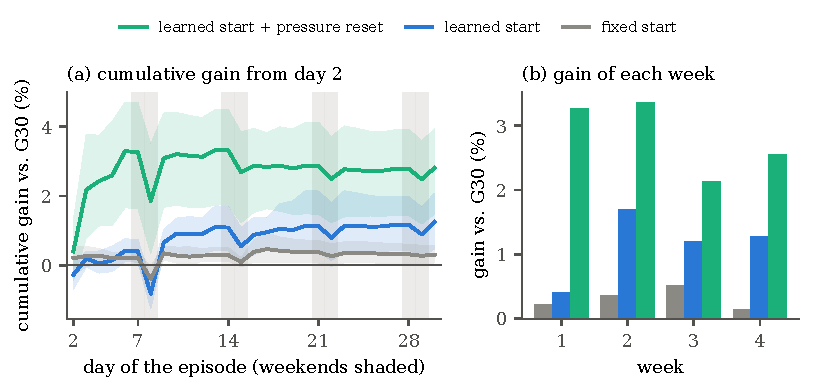
\includegraphics[width=\linewidth]{figures/fig_time_to_value_col.pdf}
\caption{Time to value on the blind set (post hoc; 30 composite episodes, each starting with no knowledge of the building). (a)
Gain over G30 accumulated up to each day, with 95\% architecture-cluster intervals; weekends shaded. Day~1, a Sunday that ends
with the first pre-start, which every start variant begins earlier than G30, is $-13.8$\% for all three and is omitted;
the dips on later Sundays have the same cause. (b) Gain of each week.}
\label{fig:timetovalue}
\end{figure}

\begin{figure}[!htbp]
\centering
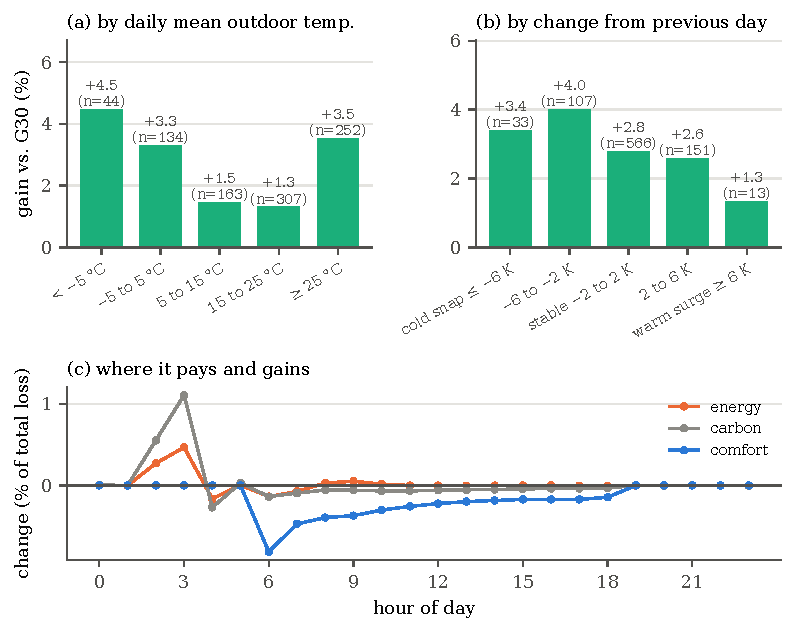
\includegraphics[width=\linewidth]{figures/fig_extremes_col.pdf}
\caption{Gain of the learning source over G30 on the blind set, per calendar day: (a) by daily mean outdoor
temperature, (b) by change of the daily mean from the previous day; (c) change of each weighted loss component by hour
of day, in \% of the total loss of G30. Panel (b) has no value for the first day of an episode; post hoc and descriptive,
and days are not independent units.}
\label{fig:error}
\end{figure}

\paragraph{Days and hours.} \Cref{fig:error} shows the gain per calendar day by outdoor temperature and by its change from the previous day, and the
change of each loss component by hour. The gain was 4.1\% and 4.2\% on the coldest and hottest 10\% of days, against
2.1\% on the others; the layer pays a little energy at 02:00--03:00 to start earlier. Of the 900 composite episode-days,
52\% improved and 2.6\% lost more than 1\% (5th and 95th percentiles $-0.23$\% and +8.9\%); most are unchanged because the
layer acts only when there is something to correct. Of the ten worst days, five are Mondays and six are US public holidays (2022-01-17, 02-21, 07-04 twice, 10-10 and 11-24),
without occupants in the simulator (summed occupancy zero, against 1,840--11,388 on the following day): neither the
controller nor the layer can know a holiday, and the earlier start adds energy that buys no comfort. The worst, Presidents'
Day 2022 in Kansas City ($-16.14$\%), followed a weekend whose daily mean rose from $-2.8$ to $+7.9\,^\circ$C: at 02:00 the
slowest blind building had a deficit of 4.4\,K and a learned time constant of about 2\,h, so the rule asked for a 5.3-h lead
and started at the 4-h bound; nobody came, and the small loss of an unoccupied day makes the relative loss large.
\paragraph{Decisions and weather surprise.}
The start is decided at night without a forecast: in 87\% of 122 decisions the predicted deficit at opening was within
0.5\,K of the actual one, and even on the mornings it missed, the day was better than with G30.
17 further starts reached the lead bound and are not judged.
\paragraph{Where the gain comes from.} \Cref{tab:occ} splits the change of the weighted loss components into occupied
and unoccupied steps.
Learned precooling on Penguin shifts some cooling to the night and saves more during the day, whereas on K07 the layer
buys comfort with a small energy cost before opening.
\begin{table}[!htbp]
\centering
\caption{Change of the weighted loss components, in \% of the comparator's total loss (blind set, composite).}
\label{tab:occ}
\small
\begin{tabular}{lrrrrr}
\toprule
& \multicolumn{2}{c}{Energy} & \multicolumn{2}{c}{Carbon} & Comfort\\
Contrast & occupied & unoccupied & occupied & unoccupied & occupied\\
\midrule
K07: G30 + layer vs.\ G30 & $-0.07$ & $+0.50$ & $-0.70$ & $+1.32$ & $-3.87$\\
Penguin + LNP vs.\ Penguin & $-2.28$ & $+0.82$ & $-0.54$ & $+0.18$ & $-0.06$\\
K07: G30 + setup vs.\ G30 & $+1.11$ & $-2.29$ & $+0.25$ & $-0.54$ & $+2.09$\\
K07: setup + learned start vs.\ setup & $-0.68$ & $+0.77$ & $-0.85$ & $+1.36$ & $-2.48$\\
\bottomrule
\end{tabular}
\end{table}

\subsection{The headroom account}\label{app:j-headroom}
\paragraph{Headroom.} Write the loss of an episode as $L = \sum_c w_c \ell_c$ over energy, carbon and comfort, let $T$ and
$O$ be the weighted losses of the terms a mechanism targets and of the others ($L = T + O$), and pool over a set $S$ of
episodes. The gain of the layer $l$ over its comparator $b$ is then exactly
\begin{equation}\label{eq:headroom}
g_S = B_S - C_S, \qquad B_S = \kappa_S\, h_S \le h_S,
\end{equation}
with the targeted share $h_S = 100 \sum_S T_b / \sum_S L_b$, the part of the targeted loss removed
$\kappa_S = \sum_S (T_b - T_l) / \sum_S T_b \le 1$, and the cost in the other terms
$C_S = 100 \sum_S (O_l - O_b) / \sum_S L_b$; hence $g_S \le h_S$ whenever $C_S \ge 0$, and $g_S$ follows $h_S$ when $\kappa_S$
and $C_S$ vary less than $h_S$. \Cref{tab:headroom} gives each term (post hoc; the neural controller with the same checks
as the others) and checks the relation of \cref{sec:depends}. Gain and share both divide by the comparator's loss,
but a permutation that keeps only this common denominator gives correlations near zero, below the interval of each observed one, and for the comfort
layer the relation also holds over architectures, without ratios and with one architecture left out (\cref{tab:headroom}). The layer removed 15--24\% of
the comfort loss on all three comfort controllers; on K07-G30 and ZT Best it removed a larger part where the share was larger,
while on Residual PPO the part removed did not rise with the share ($\rho = -0.30$), so there the association comes from the size of the headroom, and the cost in the other terms decided the two
architectures that lost (\cref{app:j-controllers}). The same architectures left comfort loss under all three ($\rho = 0.82$--$0.94$ between their per-architecture
shares), and the layer gained on the same ones ($\rho = 0.65$--$0.71$ between their per-architecture gains; with Penguin's
precooling $0.13$--$0.52$). Penguin's precooling targets terms that make up almost all of its loss, so that share bounds
little; it removed under 2\% of it, and its relation with the share is weak over architectures and without ratios. All of
this is post hoc on the frozen blind runs. The predictions registered for ZT Best and Residual PPO reuse the same 36
blind scenes: they test whether the account transfers across controllers, not whether it holds on new buildings.
\begin{table}[!htbp]
\centering
\caption{Decomposition of the blind-set gains and checks of their relation with the share of the targeted terms (post hoc).
Top: in \% of the comparator's loss, pooled over the 10 composite architectures (\cref{eq:headroom}); a positive change of
the other terms is a cost. Bottom: Spearman correlation of the episode gain with the share of the targeted terms; the null permutes the loss
reductions across episodes (10{,}000 permutations), which keeps only the denominator that gain and share have in common;
without ratios: absolute loss reduction against the absolute targeted loss; one architecture left out: the correlation over
the episodes recomputed without each architecture in turn.}
\label{tab:headroom}
\footnotesize
\setlength{\tabcolsep}{4pt}
\begin{tabular}{@{}lrrrr@{}}
\toprule
 & K07-G30 & ZT Best & Residual PPO & Penguin\\
 & + layer & + layer & + layer & + precooling\\
\midrule
Targeted terms & comfort & comfort & comfort & energy, carbon\\
Targeted share, $h$ & 15.9 & 44.2 & 22.4 & 97.2\\
Benefit, $B$ & 3.87 & 6.62 & 4.70 & 1.82\\
Cost in the other terms, $C$ & $+1.05$ & $+0.91$ & $+1.34$ & $-0.06$\\
Net gain, $g$ & 2.82 & 5.71 & 3.37 & 1.88\\
Part of it removed, $\kappa$ & 24.3 & 15.0 & 21.0 & 1.9\\
\midrule
$\rho$ over the 36 episodes & $+0.80$ & $+0.93$ & $+0.75$ & $+0.68$\\
\quad 95\% interval, by architecture & [$+0.57$, $+0.89$] & [$+0.78$, $+0.97$] & [$+0.51$, $+0.87$] & [$+0.53$, $+0.81$]\\
\quad common denominator alone, mean & $-0.09$ & $-0.18$ & $-0.12$ & $-0.04$\\
\quad\quad 95\% range & [$-0.42$, $+0.25$] & [$-0.49$, $+0.14$] & [$-0.44$, $+0.21$] & [$-0.33$, $+0.25$]\\
$\rho$ over the 12 architectures & $+0.78$ & $+0.92$ & $+0.78$ & $+0.30$\\
$\rho$ without ratios & $+0.84$ & $+0.95$ & $+0.75$ & $+0.28$\\
$\rho$, one architecture left out & $+0.77$ to $+0.83$ & $+0.91$ to $+0.94$ & $+0.72$ to $+0.78$ & $+0.65$ to $+0.73$\\
$\rho$(part removed, share) & $+0.54$ & $+0.60$ & $-0.30$ & $+0.68$\\
\bottomrule
\end{tabular}
\end{table}

\paragraph{Early indication.} The share in \cref{tab:headroom} is measured over the whole episode. To see whether a short window
indicates it in advance, three indicators were fixed from the first week (days 1--7) of G30 before this analysis was first run
(exploratory, post hoc on the blind runs): the comfort share of that week's loss, the mean distance of the zone temperatures at
each opening from their median over the occupied hours that follow, and the time from the opening until the mean zone temperature
comes within 0.5\,K of that median; the last two use sensors only. \Cref{tab:earlyind} relates them to the gain over days 8--30,
which does not overlap the window. The first-week comfort share ranked the layer's later gain almost as well as the share of the
whole episode ($\rho = 0.72$ against $0.77$; 3.95\% against 0.68\% above and below its median), whereas
the two temperature indicators did not; for the learned start alone, the temperature distance at opening split the later gain at
its median (2.48\% against 0.05\%), but its rank correlation was weak. With 10 architectures and the runs
that measured the layer, this is an indication for further study, not a validated selector; using it before the layer acts would also need a first
week without the layer to measure that share.
\begin{table}[!htbp]
\centering
\caption{Early indicators from the first week of G30 and the gain over days 8--30 (post hoc, exploratory): Spearman $\rho$ over
the 30 composite episodes with 95\% architecture-cluster intervals, its range when one architecture is left out, and $\rho$ over
the 10 architectures. The last row uses the whole episode and is not an early indicator.}
\label{tab:earlyind}
\footnotesize
\setlength{\tabcolsep}{4pt}
\begin{tabular}{lcccc}
\toprule
 & \multicolumn{3}{c}{Layer} & Learned start\\
\cmidrule(lr){2-4}\cmidrule(lr){5-5}
Indicator & $\rho$ [95\%] & one left out & architectures & $\rho$ [95\%]\\
\midrule
Comfort share of the loss & $+0.72$ $[+0.24, +0.88]$ & $+0.64$ to $+0.84$ & $+0.82$ & $+0.19$ $[-0.18, +0.46]$\\
Temperature distance at opening & $+0.23$ $[-0.09, +0.53]$ & $+0.14$ to $+0.32$ & $+0.55$ & $+0.38$ $[-0.03, +0.71]$\\
Recovery time after opening & $+0.13$ $[-0.20, +0.43]$ & $+0.06$ to $+0.26$ & $+0.41$ & $+0.08$ $[-0.17, +0.29]$\\
\midrule
Comfort share, whole episode & $+0.77$ $[+0.38, +0.90]$ & $+0.71$ to $+0.85$ & $+0.82$ & $+0.44$ $[+0.18, +0.63]$\\
\bottomrule
\end{tabular}
\end{table}

\paragraph{The objective.}
This trade pays because comfort carries 60\% of the weight: re-weighted with comfort weight $w$ and $(1-w)/2$ on energy and on
carbon, the same runs give 0.26\% with equal objective weights
and a loss below a comfort weight of 0.3 (\cref{fig:when}b); learned precooling on Penguin keeps 1.9--2.3\% across this sweep.

\subsection{Other controllers and checks of the mechanism}\label{app:j-controllers}
Each test marked registered in this subsection was frozen in a protocol before its runs (\cref{tab:registry}).

\paragraph{A trained neural controller (registered).} The public Residual PPO controller~\cite{chilton2026resppo} runs a tuned per-zone PI
rule of the ZT Best lineage with an off-hours rule, plus a residual policy trained with PPO in a chain of runs on official training
buildings and, in the last run, on 2{,}700 generated buildings, so the blind architectures are new to the layer but not necessarily
outside the network's training distribution. It has one shared network per entity type (zone, air handler, plant;
two hidden layers of 128 units), copied to every entity, so that the same weights run any building; each copy reads its own entity's
features and fixed summaries of the entities connected to it, without learned message passing. The layer was
attached unchanged: it reads and sets the rule inside the controller, and its pressure floor applies to the final command, after the
network's correction. Under a protocol frozen before any blind run (with the layer switched off the runs were bitwise identical to the
controller's own; with it on, identical up to its first action), it gained 3.37\% $[1.57, 5.22]$ over the 10 composite
architectures, 8 of 10 better (sign test $p = 0.11$: evidence of an aggregate gain more than of a gain on every
architecture) and +5.58\% on the OOD pair; two architectures lost 1.15 and 1.35\%, so the
pre-specified rule (none more than 1\% worse) failed. The gain was a comfort benefit of 4.70 points against energy and
carbon costs of 0.61 and 0.73; the controller left 22\% of its pooled blind-set loss in comfort. Of four
predictions registered before the outcome, three held: the gain rose with the controller's comfort share ($\rho = 0.75$),
the gain over all 36 episodes (3.78\%) exceeded K07's 2.69\% as its mean per-episode comfort share (21\%) exceeded
K07's 13\%, and the first-week share ranked the gain over days 8--30 ($\rho = 0.51$); the
lowest-share third gained 0.70\%, outside $\pm 0.5\%$. On six official training scenes, from buildings and
climates the network was trained on, where it leaves 2.5\% of its loss in comfort, the layer gained 0.14\%.

\paragraph{Where the neural controller gained and lost (post hoc).} Across the 12 architectures, rather than the 36 episodes of the
registered test, the gain also followed the controller's comfort share (Spearman $\rho = 0.78$). The two architectures that lost differed: on 52209 the
controller left 3.0\% of its loss in comfort, so the layer removed only 0.25 points while energy and carbon rose by 1.60;
on 52211 it removed 1.87 points of comfort loss, but energy and carbon rose by 3.0, from 7.5 more at night (00--05\,h)
only partly recovered in the morning. On the six official training scenes the pattern was the same: night-time energy and
carbon rose on all six, and comfort improved clearly only on the two scenes where the layer gained. On the leaderboard the
layer worsened the controller's score from 0.01053 to 0.01064 ($-1.0$\%), against the registered prediction of no change,
which rested on six official scenes, in sample for the network, on four of which the layer had already lost.

\paragraph{An early warning (exploratory).} Both architectures on which the layer lost had no gain in the first week
($-0.05$ and $-2.41$\%); so did one that later gained (52301, $-0.10$\%, then $+3.40$\% over days 8--30), whereas the
first-week comfort share, which ranked the later gain on K07, flagged only one of the two. A layer that switches itself off
after a first week without gain would thus have avoided both losses at the cost of that later gain. The analysis is retrospective: a deployable rule would need an observable proxy of the first-week gain and a test on new
architectures.

\paragraph{A graph network imitating the neural controller (registered).} A graph network over zones, air handlers and the plant (two rounds of message
passing) was trained to imitate the residual policy of the neural controller on the held-out and official training
buildings; on four validation episodes from other buildings it reproduced it closely ($R^2 \ge 0.97$ for every output; loss
0.9998 of the teacher's). It therefore tests the unchanged layer on a graph-structured implementation of the same policy,
not on an independent controller. With all 72 blind runs carrying the registered weights,
the unchanged layer gained 3.55\% $[1.82, 5.40]$ over the 10 composite architectures, 8 of 10 better and +5.73\% on the OOD
pair; 52209 lost 1.17\%, so the pre-specified rule failed, as on the neural controller there. The gain was a comfort benefit of
4.75 points against energy and carbon costs of 0.57 and 0.64. All four predictions registered before the outcome held: the gain
rose with the controller's comfort share ($\rho = 0.74$), the lowest-share third gained 0.48\%, within $\pm 0.5\%$, the gain
over all 36 episodes (3.96\%) exceeded K07's 2.69\% as its mean per-episode comfort share (22\%) exceeded K07's 13\%, and the first-week
share ranked the gain over days 8--30 ($\rho = 0.49$). Alone, the graph network was 0.80\% worse than the controller it
imitates ($[-1.94, +0.21]$).

\paragraph{Which rule brings the gain on the neural controller (registered).} Each rule of the layer was run alone on the neural controller's 36 blind scenes, on a different machine
from the controller alone and the full layer (such runs differ across machines by at most $10^{-6}$ per step). The pressure
reset alone gained 2.99\% $[1.60, 4.53]$ over the 10 composite architectures, all 10 better (+5.07\% on the OOD pair), and the
learned start alone 0.49\% $[-0.10, 1.03]$, 7 of 10 better; together, 3.37\%. All four registered predictions held: each rule
alone gained, both together gained at least as much as the better one, and each lowered the comfort loss (by 1.46 and 3.37
points; together 4.70). Both losses of the layer came through the start: alone it lost 1.34\% on 52209 and
1.15\% on 52211, where the reset alone gained, and added to the reset it gained 0.39\% $[-0.17, 0.92]$ on average but lost up to
1.41\%. Its earlier starts, before opening, raised energy and carbon (0.33 and 0.64 points), which on these two architectures
the comfort they bought did not repay; the reset alone would have passed the layer's pre-specified rule.

\paragraph{Learning inside the full layer (registered).} The
layer with the start's time constant fixed at 1\,h was compared with the full layer, both with the pressure reset, on the 36
blind scenes. Learning added 0.94\% $[0.10, 1.82]$ over the 10 composite architectures (7 of 10 better, exact Wilcoxon
$p = 0.084$; $-0.18\%$ on the OOD pair), so by its registered pooled criterion learning adds value inside the layer; it removed
1.50 points of comfort loss at 0.56 more in energy and carbon. In points of baseline-referenced gain, learning added 0.84 with
the reset and 0.86 without it, and the reset added 1.45 on the fixed start and 1.43 on the learned one: the two parts add up,
and neither absorbs the other. As in the start contrasts above, the evidence is stronger for the pooled gain than for every
architecture. Two episodes of the full layer re-run on the second machine matched their originals bit for bit.

\paragraph{The value of knowing the time constant early (registered).} Given each episode's final time constant from the
first day (an oracle, not deployable), the layer gained 0.02\% more ($[-0.003, +0.057]$; 6 of 9 changed composite
architectures better), 0.044\% over days 1--14 and 0.010\% over days 15--30; both registered predictions held. This is the
value of early knowledge of $\tau$ for this start rule, not an upper bound on what a different rule could gain.

\paragraph{A third rule (registered).} The Guideline~36 unoccupied setup, added to the learned start and the pressure reset with its
parameter as in the unoccupied-setup test, gained 0.38\% over the layer ($[-0.45, +1.49]$; 5 of 10 composite
architectures better, the worst $-2.46$\%): it removed 1.29 points of energy and 0.32 of carbon and added 1.23 of comfort
loss. Both registered predictions held: adding the setup had the same sign as adding it on top of the learned start alone,
and it lowered energy and carbon.

\subsection{Where each rule paid: official scenes, leaderboard and an unoccupied setup}\label{app:j-paid}
\begin{table}[!htbp]
\centering
\caption{Kaggle public leaderboard (lower is better). Scores were never used to choose a configuration.}
\label{tab:lb}
\small
\begin{tabular}{lr@{\hspace{1.6em}}lr}
\toprule
Submission & Score & Submission & Score\\
\midrule
K07, baseline $B$            & 0.01517 & G30 + learned start                     & 0.01477\\
K07, one-time gate (MG)      & 0.01549 & G30 + layer (start, pressure reset)     & 0.01477\\
K07, tuned fixed G30         & 0.01477 & G30 + unoccupied setup                  & 0.01414\\
Penguin (reproduced)         & 0.01004 & G30 + unoccupied setup + learned start  & 0.01415\\
Penguin + learned precooling & 0.01001 & Residual PPO, alone / + layer & 0.01053 / 0.01064\\
\bottomrule
\end{tabular}
\end{table}
\begin{table}[!htbp]
\centering
\caption{Which source paid where (summary of \cref{sec:results}). Gains pooled over the composite architectures; P: pre-specified, R: registered in advance, D: descriptive.}
\label{tab:when}
\footnotesize
\setlength{\tabcolsep}{4pt}
\begin{tabular}{>{\raggedright\arraybackslash}p{3.7cm}>{\raggedright\arraybackslash}p{2.6cm}>{\raggedright\arraybackslash}p{5.2cm}c}
\toprule
Situation & Source & Result & Status\\
\midrule
Buildings of the profiles' own families & one-time profile gate & $+0.504$\,pp over persistence; registered replication $+0.255$\,pp, inconclusive & P, R\\
New buildings & frozen profiles & did not transfer (held-out $-0.9$\%; leaderboard worse than $B$) & P, D\\
New buildings; controller leaves comfort loss (mean share 13--36\%) & learned start + pressure reset & $+2.82$\% (K07-G30), $+5.71$\% (ZT Best), $+3.37$\% (Residual PPO; per-architecture rule failed) & P, R\\
New buildings; controller loses mainly in energy and carbon (97\%) & learned precooling & $+1.88$\% (Penguin), all 12 architectures improved & P\\
Little loss left in comfort (official scenes, 0.2--4.6\%) & learned start + pressure reset & leaderboard unchanged (K07), 1.0\% worse (neural controller) & D, R\\
\bottomrule
\end{tabular}
\end{table}
\paragraph{Where each rule paid.} \Cref{tab:wherepaid} collects the tests of the learning source, on unseen
architectures, on the official scenes and on the leaderboard. The comfort rules gained where the controller left comfort
loss and not where it left almost none; the energy rules gained where energy could be saved at little cost in comfort.
Only the tests marked R were predicted in advance; the account of the others is post hoc.

\begin{table}[!htbp]
\centering
\caption{Where each rule paid: the tests of the learning source by controller and setting. Gains are pooled loss reductions over the episodes of the
set (leaderboard: change of the public score); P: pre-specified test; R: outcome registered in advance (as in
\cref{tab:evidence}).}
\label{tab:wherepaid}
\footnotesize
\setlength{\tabcolsep}{4pt}
\begin{tabular}{>{\raggedright\arraybackslash}p{1.9cm}>{\raggedright\arraybackslash}p{2.7cm}>{\raggedright\arraybackslash}p{2.6cm}>{\raggedright\arraybackslash}p{3.8cm}r}
\toprule
Controller & Rule(s), target & Scenes & What the controller left & Gain (\%)\\
\midrule
K07-G30 & start + reset, comfort & unseen (P) & comfort 13\% of its loss & $+2.82$\\
ZT Best & start + reset, comfort & unseen (P, R) & comfort 36\% & $+5.71$\\
Residual PPO & start + reset, comfort & unseen (R) & comfort 21\% & $+3.37$\\
Graph network (imitating it) & start + reset, comfort & unseen (R) & comfort 22\% & $+3.55$\\
Residual PPO & reset alone, comfort & unseen (R) & comfort 21\% & $+2.99$\\
Residual PPO & start alone, comfort & unseen (R) & comfort 21\%; night-time cost on two architectures & $+0.49$\\
Residual PPO & start + reset, comfort & official training scenes & comfort 2.5\% (in sample for the network) & $+0.14$\\
K07-G30 & start + reset, comfort & leaderboard & comfort 0.2--4.6\% on the official scenes & $0.00$\\
Residual PPO & start + reset, comfort & leaderboard (R: no change) & comfort 2.5\% on the official scenes & $-1.04$\\
Penguin & precooling, energy & unseen (P) & energy and carbon 97\% & $+1.88$\\
Penguin & precooling, energy & leaderboard & acted on 1 of 8 official scenes & $+0.30$\\
K07-G30 & unoccupied setup, unoccupied cooling & official scenes; leaderboard & 9--25\% unoccupied energy; acted on the two hot scenes & $+2.25$; $+4.3$\\
K07-G30 & unoccupied setup, unoccupied cooling & unseen (P, R) & saved 2.8 points, cost 3.5 (mostly comfort) & $-0.62$\\
K07-G30 + layer & unoccupied setup added & unseen (R) & over the layer & $+0.38$\\
\bottomrule
\end{tabular}
\end{table}

\paragraph{Official training scenes.} On the official training buildings the pressure reset of K07-G30 acted in 19 of
2{,}880 steps and the learned start only after cold nights, consistent with K07's unchanged five-decimal leaderboard score, though the activity on the hidden scenes is
unknown. In the warm official scenes K07 spends 9--25\% of its loss on energy during unoccupied hours, because it follows the
official unoccupied band. The Guideline~36 unoccupied cooling setpoint (32.2\,$^\circ$C) passed its gate (development
$+1.26$\%, official scenes $+2.25$\%), saving 11.4\% on the hottest official scene and nothing where nights are cool (per scene, with and without the learned
start, in \cref{tab:uns}). On that scene, in the first three occupied hours of weekdays, the zone furthest from the band was
0.57\,K outside it on average (0.22\,K without the setup) and the mean zone 0.04\,K, and the learned start changed nothing
(one scene). Learned precooling
acted in only one of eight official training scenes, where it reduced Penguin's loss by 2.7\% over ten days, so it was
expected to leave Penguin's score nearly unchanged.

\begin{table}[!htbp]
\centering
\setlength{\tabcolsep}{4pt}
\caption{Unoccupied setup on six official training scenes: gain (\%) of the setup over G30 and of the learned start on
top of it, mean night outdoor temperature ($^\circ$C) and the highest mean zone temperature when unoccupied (G30 /
setup, $^\circ$C).}
\label{tab:uns}
\footnotesize
\begin{tabular}{lrrrr}
\toprule
Scene & Setup vs.\ G30 & Learned start added & Night $T_{\mathrm{out}}$ & Max zone $T$ unoccupied\\
\midrule
building\_train\_1 / denver\_7 & $-0.00$ & $-0.00$ & 11.5 & 22.9 / 22.9\\
building\_train\_1 / fairbanks\_1 & $-0.00$ & $+0.08$ & $-21.0$ & 22.8 / 22.8\\
building\_train\_1 / phoenix\_5 & $+11.44$ & $-0.00$ & 35.9 & 25.4 / 31.8\\
building\_train\_1 / singapore\_8 & $+1.97$ & $-0.00$ & 26.3 & 25.0 / 27.1\\
building\_train\_2 / fairbanks\_2 & $-0.00$ & $-0.00$ & $-9.6$ & 22.7 / 22.7\\
building\_train\_4 / phoenix\_8 & $-0.00$ & $-0.00$ & 13.4 & 23.1 / 23.1\\
\bottomrule
\end{tabular}
\end{table}

\paragraph{Unoccupied setup on the blind set.} The setup, the setup with the learned start and the learned start alone were
compared with G30 on the blind set under a protocol fixed before any setup run on this set was read (\cref{tab:unsblind}).
Its rule for the combination against G30 (lower composite loss, most changed composite architectures better, none more
than 1\% worse) failed on the last condition and held against the setup. By term (\cref{tab:occ}), the setup saved
unoccupied energy and carbon but cost more during occupancy, mostly comfort, which the learned start more than recovered;
found by a diagnosis of the official scenes, its night saving did not cover its daytime cost on the blind set.
\begin{table}[!htbp]
\centering
\caption{Unoccupied setup on the blind set, under a protocol fixed before any setup run on this set was read: gain (\%) pooled
over the 10 composite architectures, composite architectures better of those changed, the lowest architecture gain, and the
pooled gain on the two OOD architectures. U: setup; R: learned start; UR: both.}
\label{tab:unsblind}
\small
\begin{tabular}{lrrrr}
\toprule
Contrast & Gain & Better & Worst & OOD\\
\midrule
U vs.\ G30 & $-0.62$ & 3/10 & $-5.14$ & $-2.95$\\
R vs.\ G30 & $+1.25$ & 8/10 & $-0.16$ & $+0.00$\\
UR vs.\ U & $+1.87$ & 10/10 & $+0.01$ & $+0.77$\\
UR vs.\ G30 & $+1.27$ & 7/10 & $-3.31$ & $-2.17$\\
\bottomrule
\end{tabular}
\end{table}

\paragraph{Variants that did not pass.} The K07 start attached to Penguin's pre-conditioning time lost 0.67\% in development; a first weather-clustered version of the start bounds (longer lead in deep cold) lost 0.36\% on the blind set because the safety freeze triggered in two slow buildings, and the corrected version, made after this failure and run on the same blind set, gained 0.21\% (post hoc;
\cref{tab:tests}).

%======================================================================
\section{Compute, software and licences}\label{app:compute}
%======================================================================
All runs used CPUs only: a laptop (AMD Ryzen 7 5800H), a shared workstation and Kaggle CPU notebooks; the same K07 episode of the
learning source gave bitwise-identical results on different machines; the hosted runtime of the profile study
passed a tolerance screen instead (\cref{app:execution}), and the neural controllers differ across machines by at most $10^{-6}$
per step in the reward. A 30-day episode took a median of 21--49 minutes on one
core, depending on the machine, and about 1.2\,GB of memory; the controllers needed 1--4\,ms per step, so the simulator
dominates. The simulator is the evaluation kit of the Smart Buildings Challenge~\cite{goldfeder2026challenge}, identified by
the SHA-256 of its evaluation script (\texttt{947c968ce3a891da\allowbreak 8334b7504ac0e7b4\allowbreak 5bd14fe13400f013\allowbreak 6df49825d5247792}); every run records that hash and the hashes of its runner,
controller code and scenario configuration, and most record the NumPy version (2.0 or 2.1). K07, ZT Best, Penguin (which builds on a public controller by Daniel
Wu~\cite{wu2026cpub}) and the Residual PPO controller are public notebooks under the Apache License~2.0~\cite{malyshev2026k07,malyshev2026zt,penguin2026deep,chilton2026resppo}; weather comes from
NOAA's Integrated Surface Database~\cite{smith2011isd}. The competition data are licensed CC BY-NC-SA 4.0. Bootstrap and permutation tests use fixed seeds.

\paragraph{Reproducing the learning-source result.} Average the absolute reward of G30 and of the layer over the 8,640 steps of
each blind episode, pool both over the 30 episodes of the 10 composite architectures and compute
$100\,(1 - \sum L_{\mathrm{layer}} / \sum L_{\mathrm{G30}}) = 2.82\%$; resampling the composite architectures 3,000 times with a
fixed seed gives $[1.48, 3.94]$.
